%==========================================================================
%  Reading Note: Surrogate-Based Forward Modeling for Exoplanet
%  Atmospheric Retrievals
%
%  May 2026 -- filled-in version of the reading-phase skeleton.
%==========================================================================

\documentclass[11pt,a4paper]{article}

\usepackage[utf8]{inputenc}
\usepackage[T1]{fontenc}
\usepackage{lmodern}
\usepackage[margin=2.5cm]{geometry}
\usepackage{amsmath,amssymb,amsthm}
\usepackage{mathtools}
\usepackage{bm}
\usepackage{xcolor}
\usepackage{hyperref}
\usepackage{enumitem}
\usepackage{booktabs}
\usepackage{parskip}
\usepackage{graphicx}

% ==== dataset dimensions ====
\newcommand{\nHF}{97}          % high-fidelity spectra
\newcommand{\nLFpaired}{97}    % paired LF (input-matched to HF)
\newcommand{\nLFtenk}{10000}   % decoupled 10k LF design
\newcommand{\nwl}{195}         % wavelength points
\newcommand{\wlmin}{2.458}     % um
\newcommand{\wlmax}{11.750}    % um

% ==== HF-LF correlation (paired 97-row LF) ====
\newcommand{\globalr}{0.900}       % global Pearson r
\newcommand{\persampmean}{0.991}   % per-sample r: mean
\newcommand{\persampmin}{0.895}    % per-sample r: min
\newcommand{\persampmax}{0.999}    % per-sample r: max (>0.999)
\newcommand{\perwlmean}{0.538}     % per-wavelength r: mean
\newcommand{\perwlmin}{0.212}      % per-wavelength r: min
\newcommand{\perwlmax}{0.825}      % per-wavelength r: max
\newcommand{\perwlminlam}{4.29}    % um, location of minimum (CO2 band)
\newcommand{\persampFThreeTwoTwo}{0.980} % per-sample r, F322W2 (2.4-4 um)
\newcommand{\persampFFourFourFour}{0.913} % per-sample r, F444W (4-5 um)
\newcommand{\persampMIRI}{0.994}          % per-sample r, MIRI LRS (5-12 um)

% --- helper commands (kept for traceability against the skeleton) -----
\newcommand{\fillin}[1]{{\color{red}\textbf{[FILL:}\textit{ #1\,}\textbf{]}}}
\newcommand{\researchq}[1]{%
  \par\smallskip\noindent
  \textbf{\textcolor{blue}{Research question.}}\,\textit{#1}\par\smallskip}
\newcommand{\thref}[1]{{\color{teal}\textit{Thesis: #1}}}
\newcommand{\litref}[1]{{\color{violet}\textit{See: #1}}}
% ----------------------------------------------------------------------

\hypersetup{colorlinks=true,linkcolor=blue,urlcolor=blue,citecolor=blue}

% Convenient notation macros
\newcommand{\xv}{\bm{x}}
\newcommand{\yv}{\bm{y}}
\newcommand{\bz}{\bm{z}}          % spectral features z = Psi(y)
\newcommand{\bh}{\bm{h}}          % vector-valued GP map
\newcommand{\boldeta}{\bm{\eta}}  % regression noise
\newcommand{\bOmega}{\bm{\Omega}} % noise covariance
\newcommand{\Rp}{R_{\!P}}
\newcommand{\logg}{\log g}
\newcommand{\Tint}{T_{\mathrm{int}}}
\newcommand{\Kzz}{\log K_{zz}}
\newcommand{\fhr}{f}
\newcommand{\XC}{\log X_{\mathrm{C}}}
\newcommand{\XO}{\log X_{\mathrm{O}}}
\newcommand{\XN}{\log X_{\mathrm{N}}}
\newcommand{\XS}{\log X_{\mathrm{S}}}
\newcommand{\yhf}{y^{\mathrm{HF}}}
\newcommand{\ylf}{y^{\mathrm{LF}}}
\newcommand{\ymf}{y^{\mathrm{MF}}}
\newcommand{\R}{\mathbb{R}}
\newcommand{\E}{\mathbb{E}}
\newcommand{\GP}{\mathcal{GP}}
\newcommand{\N}{\mathcal{N}}
\newcommand{\T}{^{\!\top}}
\newcommand{\bth}{\bm{\theta}}
\newcommand{\bx}{\bm{x}}
\newcommand{\bxprime}{\bm{x}'}
\newcommand{\by}{\bm{y}}
\newcommand{\bff}{\bm{f}}
\newcommand{\bK}{\bm{K}}
\newcommand{\bB}{\bm{B}}
\newcommand{\bW}{\bm{W}}
\newcommand{\bmu}{\bm{\mu}}
\newcommand{\bSigma}{\bm{\Sigma}}
\newcommand{\bvarepsilon}{\bm{\varepsilon}}

\title{Reading Note: GP-Based Forward Modeling for\\Exoplanet Atmospheric Retrievals}
\author{Camilla Andreozzi}
\date{May 2026}

\begin{document}
\maketitle

\begin{abstract}
The objectives of this note are: (i)~explicit the structure of the high-fidelity (HF),
low-fidelity (LF), and multi-fidelity (MF) constructions; (ii)~flag open
questions to be resolved before the modeling phase begins; (iii)~ define further modelling strategies.
\end{abstract}

\tableofcontents
\bigskip

%==========================================================================
\section{Introduction}
%==========================================================================
% \researchq{What problem does this project address, why is the surrogate approach
% unavoidable, and what specifically will we contribute beyond the thesis?}

\subsection{Scientific Framework: Atmospheric retrieval as Bayesian inversion}

An atmospheric retrieval is the inverse problem of inferring a vector $\theta$ of atmospheric parameters from an observed emission spectrum. The emission spectrum of a transiting exoplanet encodes its composition, its vertical thermal structure, and, through disequilibrium chemistry, the strength of vertical mixing. Writing $M(\theta)$ for the forward model that maps parameters to a predicted spectrum and $\yv_{\mathrm{obs}}$ for the
observed spectrum, the retrieval is the posterior
\[
p( \theta \mid \yv_{\mathrm{obs}}) \;\propto\;
p(\yv_{\mathrm{obs}}\mid\theta)\,p(\theta),
\]
with $p(\yv_{\mathrm{obs}}\mid\theta)$ a Gaussian likelihood built around $M(\theta)$ under the assumption of independent observational noise.
% \thref{Chapter 1, especially the framing of retrieval as Bayesian
% inference (pp.~2--4).}\\
% \litref{Madhusudhan, N.~(2018), ``Atmospheric Retrieval of Exoplanets,''
% in \emph{Handbook of Exoplanets} --- the standard review.}

Standard physical techniques allow for iterative loop that eventually provide with an estimate of the forward map. However, a single evaluation of a self-consistent HF forward model takes several hours to about a day, because the chemistry and thermal-structure modules are mutually iterated for consistency.
Bayesian inference over a $9$-dimensional parameter space requires $\mathcal{O}(10^{5}\!-\!10^{7})$ forward evaluations, which corresponds to roughly $10^{2}$ CPU years even at the optimistic ``one HF call per hour'' rate. A surrogate $\hat M$ that emulates $M$ in milliseconds is therefore needed for an efficient inference.\\
% \thref{Chapter 1 closing paragraphs; Chapter 3 introduction (p.~13).}

\subsection{Scope of the project}

The dataset comprises $N_{H}=97$ HF runs produced by Latin-hypercube sampling on a $9$-dimensional input space, a much larger set of $N_{L}=10\,000$ LF runs on an enlarged Latin-hypercube design of the same $9$-dimensional space (with the $97$ HF inputs retained as a nested subset, $\bm{X}_{H}\subset\bm{X}_{L}$), an emission spectrum discretised to $m=195$ wavelength bins, and one observed JWST spectrum of WASP-80b
(NIRCam F322W2 at $2.4$--$4\,\mu$m, NIRCam F444W at $4$--$5\,\mu$m, and MIRI LRS at $5$--$12\,\mu$m; the sampled grid spans $2.46$--$11.75\,\mu$m). Crucially, the LF and HF design matrices no longer coincide: the cheap LF simulator is evaluated far more densely than the expensive HF one, $\bm{X}_{L}\neq\bm{X}_{H}$, which restores the usual multi-fidelity advantage of using abundant low-cost evaluations to explore the input space. The first objective of this project is to construct an accurate but
computationally cheap surrogate for the expensive HF forward map
\[
x \longmapsto y_{\mathrm{HF}}(x),
\]
using the available LF information to improve prediction of the HF
emission spectra. The quality of the surrogate will be assessed by
validating its predictions against held-out or cross-validated HF
spectra.

The second objective is to determine whether improved spectral
prediction also translates into a more reliable Bayesian inversion.
Since the surrogate enters directly into the likelihood of the inverse
problem, improvements in predictive accuracy and uncertainty
quantification should lead to better-calibrated posterior distributions
over the atmospheric parameters; see
Section~\ref{sec:bayesian-inversion}.

%\textcolor{red}{should the project include the full Bayesian inversion step, or should the main focus be restricted to fitting and validating the Gaussian-process multi-fidelity surrogate for the emission spectra?}

%ideally both, but we should first focus on the first step

\subsubsection*{Problem Formulation}

We observe an exoplanet emission spectrum; we want to infer the hidden atmospheric and planetary parameters that generated it; and we use surrogate models and Bayesian retrieval to resolve this inverse problem.
The only available observation data is the emission spectrum of the exoplanet. This spectrum consists of eclipse-depth measurements at fixed wavelength bins,
\[
y_{\mathrm{obs}}
=
\bigl(y_{\mathrm{obs},1},\ldots,y_{\mathrm{obs},m}\bigr)^\top
\in \mathbb{R}^m,
\]
where each component \(y_{\mathrm{obs},j}\) denotes the measured eclipse depth at wavelength \(\lambda_j\), with \(m=195\) wavelength bins.

The latent quantity of scientific interest is the vector of atmospheric and planetary parameters
\[
\theta
=
\left(
R_P,\log g,T_{\mathrm{int}},\log K_{zz},f,
\log X_C,\log X_O,\log X_N,\log X_S
\right)^\top
\in \mathcal{X}\subset \mathbb{R}^9.
\]
\label{sec:what}



These parameters describe, respectively, the planetary radius, surface gravity, internal temperature, vertical mixing strength, heat redistribution efficiency, and elemental abundance parameters for carbon, oxygen, nitrogen, and sulfur. They are not directly observable from the telescope data; instead, they must be inferred indirectly from the measured spectrum. The components, with their physical role and the Latin Hypercube Sampling / prior bounds
read off Table \ref{tab:inputs} of the thesis, are summarised below.


\begin{center}
\label{tab:inputs}
\begin{tabular}{@{}l l l l@{}}
\toprule
Symbol & Meaning & Units & Bounds (LHS = prior)\\
\midrule
$\Kzz$   & eddy-mixing coefficient (log) & cm$^{2}$\,s$^{-1}$ & $[8.0,\,11.5]$ (const.\ w/ altitude)\\
$\Rp$    & planetary radius              & $R_{\mathrm{J}}$   & narrow Gaussian, lit.\ value\\
$\Tint$  & internal temperature          & K                  & $[30,\,400]$\\
$\XC$    & log carbon abundance          & dex                & $[-12,\,-1]$\\
$\XN$    & log nitrogen abundance        & dex                & $[-12,\,-1]$\\
$\XO$    & log oxygen abundance          & dex                & $[-12,\,-1]$\\
$\XS$    & log sulfur abundance          & dex                & $[-12,\,-1]$\\
$\logg$  & surface gravity (log)         & cgs                & narrow Gaussian, lit.\ value\\
$\fhr$   & heat-redistribution factor    & dimensionless      & $[0.25,\,2/3]$\\
\bottomrule
\end{tabular}
\end{center}

The LHS design domain and the priors used in the Bayesian inversion
coincide exactly. 

The physical forward direction is
\[
\theta
\longmapsto
y_{\mathrm{HF}}(\theta),
\]
\begin{equation}
    \label{eq:ammotelodico}
    y_{HF}:\mathbb{R}^9\longrightarrow\mathbb{R}^{195}
\end{equation}
where \(y_{\mathrm{HF}}(\theta)\) denotes the high-fidelity emission spectrum predicted by a physically self-consistent atmospheric model. 

The forward model returns, for each input $\xv$, an emission spectrum
operationalised as eclipse depth on a \emph{fixed} wavelength grid:
\[
    \yv(\xv) \;=\; \bigl(d_{1}(\xv),\,\dots,\,d_{N}(\xv)\bigr)^{\!\top}
    \;\in\; \mathbb{R}^{N},
    \qquad N=195,\quad d_{j}(\xv) = d(\lambda_{j};\xv).
\]
%Wavelength should not be considered a regression input: it functions as the index of the response vector.
The grid contains three JWST instrument modes: $103$ NIRCam~F322W2 bins on $[2.4575,\,3.9875]\,\mu$m, $65$ NIRCam~F444W bins on $[4.0025,\,4.9625]\,\mu$m, and $27$ MIRI~LRS bins on $[5.25,\,11.75]\,\mu$m. The two NIRCam modes both use fine bins of width $\Delta\lambda=0.015\,\mu$m, while the MIRI~LRS bins have width $\Delta\lambda=0.25\,\mu$m. Thus a spacing-based split reveals only the NIRCam--MIRI grid discontinuity near $5\,\mu$m; the F322W2--F444W boundary must be assigned explicitly at $4\,\mu$m. The HF, LF, and observed spectra share this grid. A visualisation of the spectra can be seen in Figure~\ref{fig:hf_lf_observed}.

The statistical inverse problem is to infer
\[
p(\theta \mid y_{\mathrm{obs}})
\propto
p(y_{\mathrm{obs}}\mid \theta)\,p(\theta).
\]
For any proposed atmospheric parameter vector \(\theta\), a forward model predicts a corresponding emission spectrum
\[
\widehat y(\theta)
=
\bigl(\widehat y_1(\theta),\ldots,\widehat y_{195}(\theta)\bigr)^\top.
\]
The likelihood then measures how close this predicted spectrum is to the observed spectrum \(y_{\mathrm{obs}}\). In an ideal setting, the prediction would come from the high-fidelity simulator,
\[
\widehat y(\theta)=y_{\mathrm{HF}}(\theta).
\]
However, because the high-fidelity simulator is too expensive to evaluate repeatedly during Bayesian sampling, it is replaced with a surrogate forward model.


The central research question can therefore be stated as follows:

\begin{quote}
Can one construct a fast surrogate forward model that approximates a computationally expensive, physically and chemically self-consistent high-fidelity atmospheric simulator accurately enough to enable Bayesian retrieval of exoplanet atmospheric parameters from JWST emission spectra?
\end{quote}

That is, we study if the data-expensive mapping
\[
\theta \mapsto y_{\mathrm{HF}}(\theta)
\]
can be replaced by a computationally cheap surrogate approximation
\[
\widehat{y}(\theta) \approx y_{\mathrm{HF}}(\theta),
\]
while preserving sufficient physical accuracy for posterior inference:
\[
p(\theta \mid y_{\mathrm{obs}})
\approx
\hat{p}(\theta \mid y_{\mathrm{obs}})
\approx \hat{\mathrm{M}}(\theta)p(\theta).
\],
where \(\hat{\mathrm{M}}(\theta)\) represents our best try at estimating the likelihood of the emission spectrum.

Finally, it is worth noting that the discretisation into $m=195$ wavelength
bins is a feature of the observational setup, not of the forward problem
itself: the underlying emission spectrum is a smooth function of wavelength.
In Gaussian-process notation one can therefore regard the forward model as a
map into an (infinite-dimensional) function space,
\[
    f:\mathbb{R}^{9}\longrightarrow\mathbb{R}^{\infty},
    \qquad
    \theta\longmapsto f(\theta)(\,\cdot\,),
\]
where $f(\theta)(\lambda)$ denotes the predicted eclipse depth at an arbitrary
wavelength $\lambda$, and the $195$ bins are recovered through a sampling
(observation) operator
\[
    S:\mathbb{R}^{\infty}\longrightarrow\mathbb{R}^{195},
    \qquad
    \bigl(Sf(\theta)\bigr)_j = f(\theta)(\lambda_j),
    \quad j=1,\ldots,195 .
\]
The finite-dimensional map $y_{\mathrm{HF}}=S\circ f$ used above is thus only
one particular discretisation of this continuous model. This functional
viewpoint is agnostic to the choice of wavelength grid and lets us treat the
Gaussian-process surrogate and the PCA-based output reduction as different
finite-rank approximations of the same underlying smooth map $f$.


\subsubsection*{Atmospheric assumptions held fixed}
The atmosphere is taken as \emph{cloud-free}; the stellar spectrum is the precomputed PHOENIX model for the host star; \emph{petitRADTRANS} is the common radiative-transfer engine for both fidelities, so radiative-transfer error cancels between HF and LF; the LF chemistry is reduced to the six species 
$\mathcal{M} = \{\mathrm{H_{2}O},\mathrm{CO},\mathrm{CO_{2}},
\mathrm{CH_{4}},\mathrm{NH_{3}},\mathrm{SO_{2}}\}$,
whereas the HF model uses the full SNCHO network.\\
% \thref{Section 2.3 (cloud-free justification); Section 4.4.1 (LF
% chemistry list, p.~32).}

%==========================================================================
\section{Proposed Methodology}
\label{sec:gpmf}

%==========================================================================
% \researchq{Can we replace the staged pipeline with a single autoregressive
% Gaussian process in a shared spectral subspace, and what would change?}

\subsection{Multifidelity GPs}

The multifidelity GP model couples a low-fidelity and a
high-fidelity scalar process through
\[
    f_{HF}(x)
    =
    \rho\, f_{LF}(x) + \delta(x),
\]
with
\[
    f_{L}(x) \sim \mathcal{GP}\left(0, k_{L}(x,x')\right),
\]
and
\[
    \delta(x) \sim \mathcal{GP}\left(0, k_{\delta}(x,x')\right),
\]
and scaling factor \(\rho \in \mathbb{R}\) (or, in extensions,
\(\rho(x)\)).
Assuming centering of the data, the corresponding joint prior is
\[
    \begin{pmatrix}
        f_{L}(x) \\
        f_{H}(x)
    \end{pmatrix}
    \sim
    \mathcal{GP}
    \left[
    \begin{pmatrix}
        0 \\
        0
    \end{pmatrix},
    \begin{pmatrix}
        k_{L} & \rho\, k_{L} \\
        \rho\, k_{L} & \rho^{2} k_{L} + k_{\delta}
    \end{pmatrix}
    \right].
\]



Noisy training observations at the two fidelity levels are
\[
    y_{i}^{L}
    =
    f_{L}(x_{i}^{L}) + \varepsilon_{i}^{L},
    \qquad
    y_{i}^{H}
    =
    f_{H}(x_{i}^{H}) + \varepsilon_{i}^{H},
\]
with
\[
    \varepsilon_{i}^{L} \sim \mathcal{N}\left(0, \sigma_{L}^{2}\right),
    \qquad
    \varepsilon_{i}^{H} \sim \mathcal{N}\left(0, \sigma_{H}^{2}\right).
\]

The kernel adopted for every GP in this note is the squared-exponential
(Gaussian) kernel with automatic relevance determination (ARD), i.e.\ a
separate length-scale $\ell_r$ for each of the nine input dimensions. This is
the default choice throughout: the same ARD form is used for the low-fidelity
process, for the discrepancy, and across all three modelling options of
Section~\ref{sec:gpmf}, with only its inputs and the number of length-scales
changing (e.g.\ a tenth, wavelength length-scale is added in Model~2). On the
nine-dimensional atmospheric input space it reads
\[
    k_{L}(x,x')
    =
    \sigma^{2}_{L}
    \exp
    \left[
    -\frac{1}{2}
    \sum_{r=1}^{9}
    \frac{(x_{r}-x'_{r})^{2}}{\ell^{2}_{L,r}}
    \right],
\]
and
\[
    k_{\delta}(x,x')
    =
    \sigma^{2}_{\delta}
    \exp
    \left[
    -\frac{1}{2}
    \sum_{r=1}^{9}
    \frac{(x_{r}-x'_{r})^{2}}{\ell^{2}_{\delta,r}}
    \right].
\]
The length-scale \(\ell_{r}\) measures how sensitive the response is to
the \(r\)-th atmospheric input. A short length-scale means that small
changes in that parameter produce large output changes; a long
length-scale means that the response is relatively insensitive to that
parameter. This is precisely the ``automatic relevance determination''
property: the fitted $\ell_{1:9}$ rank the atmospheric parameters by their
influence on the spectrum, which is a useful by-product of the kernel choice.
The model hyperparameters are
\[
    \Theta
    =
    \left\{
    \rho,
    \sigma^{2}_{L},
    \sigma^{2}_{\delta},
    \ell_{L,1:9},
    \ell_{\delta,1:9},
    \sigma^{2}_{L},
    \sigma^{2}_{H}
    \right\},
\]
and can be estimated by maximizing the marginal likelihood, a full Bayesian hyperprior treatment, or via cross validation.

Stacking the LF and HF observations into a single vector
\(y=(y^{L\top},y^{H\top})^{\top} \in \mathbb{R}^{N_{L}+N_{H}}\), the
marginal distribution of the training data is Gaussian,
\[
    y
    \sim
    \mathcal{N}
    \left(
    \mathbf{0},
    K\!\left(x_{\mathrm{tr}}, x_{\mathrm{tr}};\Theta\right)
    +
    \Sigma_{\mathrm{noise}}
    \right),
\]
where \(K\) is the joint covariance built from the \(2\times 2\) kernel
block above and
\(\Sigma_{\mathrm{noise}}
=\mathrm{diag}\!\left(\sigma_{L}^{2}I_{N_{L}},\,
\sigma_{H}^{2}I_{N_{H}}\right)\).
For a new input \(x_{\ast}\), the posterior predictive distribution of
the high-fidelity response is Gaussian in closed form,
\[
    f_{H}(x_{\ast})\mid \mathcal{D}
    \sim
    \mathcal{N}
    \left(
    \mu^{\ast}(x_{\ast}),
    \sigma^{\ast 2}(x_{\ast})
    \right),
\]
where \(\mathcal{D}\) denotes the available LF and HF training data.


\subsection{Our setting: $\R^{9} \to \R^{195}$ multifidelity GP}
\label{sec:MF}

\paragraph{Set-up.}
Inputs $\bth \in \R^{9}$ as before. Outputs are now \emph{vector-valued} spectra at a fixed wavelength grid $(\lambda_{1},\ldots,\lambda_{195})$:
\[
\bff_{L}:\R^{9}\to\R^{195}, \qquad \bff_{H}:\R^{9}\to\R^{195}.
\]
Training data are now available at two distinct fidelities and on two
\emph{different} designs:
\[
\mathcal{D}_{H} = \bigl\{(\bth_{i}^{H},\, \by_{i}^{H})\bigr\}_{i=1}^{N_{H}}, \quad
\by_{i}^{H} \in \R^{195}, \quad N_{H}=97,
\]
\[
\mathcal{D}_{L} = \bigl\{(\bth_{i}^{L},\, \by_{i}^{L})\bigr\}_{i=1}^{N_{L}}, \quad
\by_{i}^{L} \in \R^{195}, \quad N_{L}=10\,000.
\]
Denoting the input design matrices
\[
\bm{X}_{H} = \bigl[\bth_{1}^{H},\ldots,\bth_{N_{H}}^{H}\bigr]\T \in \R^{N_{H}\times 9},
\qquad
\bm{X}_{L} = \bigl[\bth_{1}^{L},\ldots,\bth_{N_{L}}^{L}\bigr]\T \in \R^{N_{L}\times 9},
\]
the LF design is a much denser Latin-hypercube sampling of the same
$9$-dimensional space, in which the HF design is \emph{nested}:
\begin{equation}
N_{L} \;=\; 10\,000 \;\gg\; N_{H} \;=\; 97,
\qquad
\bm{X}_{H} \;\subset\; \bm{X}_{L},
\qquad
\bm{X}_{L} \;\neq\; \bm{X}_{H}.
\label{eq:design_nested}
\end{equation}
Because the HF inputs form a subset of the LF design, at every HF input
$\bth_{i}^{H}$ a matched LF evaluation is available, so the discrepancy
$\bm{\delta}_{i} = \by_{i}^{H} - \rho\,\by_{i}^{L}$ remains directly observable
on the $N_{H}=97$ co-located points; the remaining $N_{L}-N_{H}$ LF runs carry
no matched HF counterpart.

\medskip
\noindent Unlike a co-located design, the enlarged LF set adds genuine
probabilistic spatial coverage of the $9$-dimensional input space. This is the
usual motivation for multi-fidelity modelling: the cheap LF simulator is
sampled far more densely than the expensive HF one, so the LF data inform the
surrogate both through the discrepancy estimated at the nested HF points and
through extended exploration of the input space well beyond the $97$ HF
locations.

\subsection{Modelling}

We pursue three modelling options, developed in
Sections~\ref{subsec:model1}--\ref{subsec:model3-role-switched}: an independent
per-wavelength multi-fidelity GP (Model~1), a single GP with wavelength promoted
to an additional input (Model~2), and a role-switched conditional surrogate that
learns the inverse map directly (Model~3). Two cross-cutting choices recur in all
three and are therefore treated separately rather than re-derived for each model.
The first is the parametrisation of the scaling factor $\rho$: it may be fitted
either as a single global scalar shared across all wavelengths, or as a smoothly
varying function $\rho(\lambda)$ expanded on a spline basis. These two
correlation-modelling methodologies are developed in
Section~\ref{subsec:correlation-modelling}. The second is that the HF--LF
correlation is not homogeneous across the spectrum: the observed spectrum is
stitched from three JWST instrument modes (NIRCam~F322W2, NIRCam~F444W, MIRI~LRS)
whose resolutions, noise, and HF--LF agreement differ markedly, so any of the
three models must be allowed to express \emph{different correlation structure in
different instrument bands} --- whether through a wavelength-dependent $\rho$ and
an instrument-aware wavelength kernel, or by fitting a separate model per
instrument. The empirical evidence for this instrument-driven correlation
structure is given in the preliminary results
(Section~\ref{subsec:instrument-structure}).

%1. Model 1: we fit 195 separate models based on the 97 outputs
% =====================================================================
%  Model 1 : Independent per-wavelength (pixel-basis) multifidelity GP
%  Drop-in for Section 3.3 (Modelling) of the working note.
%  Assumes the note's preamble (amsmath, amssymb) and its established
%  notation:  theta in R^9 ,  f_L , f_H , rho ,  n = 97 ,  m = 195 ,
%  the co-located design  X_L = X_H , and the SE kernel of Sec. 3.1.
% =====================================================================

\subsection{Model 1: independent per-wavelength multifidelity GP}
\label{subsec:model1}

We construct the first modelling approach as follows. Identify the $j$-th output coordinate with the eclipse depth in bin $\lambda_j$ and
treat it as a scalar response. For each $j=1,\dots,m$ we instantiate the
two-level scalar model of Section \ref{sec:MF} independently,
\begin{equation}
  f_{H,j}(\boldsymbol\theta)
    \;=\; \rho_j\, f_{L,j}(\boldsymbol\theta) \;+\; \delta_j(\boldsymbol\theta),
  \qquad j = 1,\dots,m,
\end{equation}
with mutually independent processes
\begin{equation}
  f_{L,j}\sim\mathcal{GP}\!\bigl(0,\,k_{L,j}\bigr),
  \qquad
  \delta_{j}\sim\mathcal{GP}\!\bigl(0,\,k_{\delta,j}\bigr),
\end{equation}
independent across $j$ and between level and discrepancy. Every bin therefore
carries its own low-fidelity kernel
$k_{L,j}$ and its own discrepancy kernel $k_{\delta,j}$; the spectrum is never
modelled jointly. Equivalently, the vector map $f_H:\mathbb{R}^{9}\to\mathbb{R}^{m}$
is approximated coordinate-wise in the standard (pixel) basis
$\{\mathbf{e}_1,\dots,\mathbf{e}_m\}$ of $\mathbb{R}^{m}$, one GP per coefficient.
The wavelength $\lambda_j$ is a fixed index selecting which GP is read, not a covariate.
The choice and parametrisation of the scaling factor $\rho$ are treated separately in Section~\ref{subsec:correlation-modelling}.

Because the HF design is nested in the LF design (Eq.~\ref{eq:design_nested},
$\bm{X}_{H}\subset\bm{X}_{L}$), at every HF training input $\boldsymbol\theta_i^{H}$ both
fidelities are observed, so the per-bin discrepancy is \emph{directly observable}
on the $N_{H}=97$ co-located points,
\begin{equation}
  \delta_j(\boldsymbol\theta_i^{H})
    \;=\; y^{H}_{i,j} \;-\; \rho_j\, y^{L}_{i,j},
  \qquad i = 1,\dots,N_{H} .
\end{equation}
This permits a recursive scheme: estimate $\rho_j$ and the LF
process from the full LF sample $\{(\boldsymbol\theta_i^{L},\,y^{L}_{i,j})\}_{i=1}^{N_{L}}$,
form the observed residuals at the nested HF points, and fit $\delta_j$ to them,
avoiding the coupled joint inverse.

As elsewhere in this note, the kernel at each GP level is the squared-exponential
ARD kernel (one length-scale per input dimension):
\begin{equation}
  k_{L,j}(\boldsymbol\theta,\boldsymbol\theta')
    = \sigma^2_{L,j}\exp\!\Bigl[-\tfrac12\textstyle\sum_{r=1}^{9}
      \tfrac{(\theta_r-\theta'_r)^2}{\ell^{2}_{L,j,r}}\Bigr],
  \qquad
  k_{\delta,j}(\boldsymbol\theta,\boldsymbol\theta')
    = \sigma^2_{\delta,j}\exp\!\Bigl[-\tfrac12\textstyle\sum_{r=1}^{9}
      \tfrac{(\theta_r-\theta'_r)^2}{\ell^{2}_{\delta,j,r}}\Bigr],
\end{equation}
the per-bin hyperparameter set is
\begin{equation}
  \Theta_j=\bigl\{\rho_j,\;\sigma^2_{L,j},\;\boldsymbol\ell_{L,j,1:9},\;
    \sigma^2_{\delta,j},\;\boldsymbol\ell_{\delta,j,1:9},\;
    \sigma^2_{nL,j},\;\sigma^2_{nH,j}\bigr\},
\end{equation}
fitted by marginal-likelihood maximisation (\textcolor{red}{I suppose we do marginal-likelihood}) independently for each $j$. The full model carries $m=195$ such sets, i.e.\ of order
$195\times(2\!\cdot\!10+1)\approx 4\times10^{3}$ hyperparameters; the LF-level parameters are estimated from the full $N_{L}=10\,000$ LF sample, while the discrepancy parameters rely on the $N_{H}=97$ nested HF points.

For a proposed input $\boldsymbol\theta_\ast$ the HF posterior at each bin is
Gaussian in closed form,
\begin{equation}
  f_{H,j}(\boldsymbol\theta_\ast)\,\big|\,\mathcal{D}
    \;\sim\; \mathcal{N}\!\bigl(\mu_j(\boldsymbol\theta_\ast),\,
                                 s^2_j(\boldsymbol\theta_\ast)\bigr),
\end{equation}
and the predicted spectrum is assembled by stacking the $m$ posterior means against
the fixed grid,
\begin{equation}
  \hat{\mathbf{y}}(\boldsymbol\theta_\ast)
    = \bigl(\mu_1(\boldsymbol\theta_\ast),\dots,\mu_m(\boldsymbol\theta_\ast)\bigr)^{\!\top}
    \in\mathbb{R}^{m}.
\end{equation}
Plotted against $(\lambda_1,\dots,\lambda_m)$ this vector \emph{is} the predicted emission spectrum: a stacking of independent bin-wise predictions. 

Assumed independence across $j$ makes the joint HF predictive covariance diagonal,
\begin{equation}
  \mathrm{Cov}\!\bigl(\hat{\mathbf{y}}(\boldsymbol\theta_\ast)\bigr)
    = \mathrm{diag}\!\bigl(s^2_1(\boldsymbol\theta_\ast),\dots,
                            s^2_m(\boldsymbol\theta_\ast)\bigr),
\end{equation}
which feeds directly into the Gaussian likelihood of Section~5.1 with
\begin{equation}
  M_j(\boldsymbol\theta) = \mu_j(\boldsymbol\theta),
  \qquad
  \sigma^2_{\mathrm{surrogate},j} = s^2_j(\boldsymbol\theta).
\end{equation}

\paragraph{Issues:}
\begin{itemize}
    \item This independence between outputs makes the diagonal predictive covariance encode no cross-bin correlation, although the underlying map
    $S\circ f$ is the discretisation of a \emph{smooth} function $f$ and neighbouring bins are tightly coupled
    within molecular bands. This is
    harmless under the present diagonal likelihood, but it stresses even more the likelihood independence assumption.
    \item About ten hyperparameters per bin are estimated from only $n=97$ points. 
    \item Each bin's mean and variance are free to disagree with their neighbours, so reconstructed spectra and their uncertainty bands can be non-smooth even though $f(\boldsymbol\theta)(\cdot)$ is smooth in wavelength.
\end{itemize}

% ============================================================
% Model 2: wavelength as an additional input
% ============================================================

\subsection{Model 2: wavelength as an additional input}
\label{subsec:model2-wavelength-input}

Model~1 treats the wavelength index \(j\) as fixed and fits one scalar
multi-fidelity GP for each wavelength bin \(\lambda_j\). This is natural
from the discretised point of view, where the spectrum is represented as
a vector in \(\mathbb R^m\), with \(m=195\). However, physically the
forward model is better understood as producing a smooth emission spectrum
as a function of wavelength. The discretisation into \(m\) bins is induced
by the observational wavelength grid.

We therefore consider an alternative formulation in which wavelength is
included as an additional input variable. Define the augmented input
\[
    z = (\theta,\lambda)
    \in
    \mathcal Z
    :=
    \mathcal X \times \Lambda
    \subset \mathbb R^{10},
\]
where \(\theta \in \mathcal{X}\subset \mathbb{R}^9\) is the vector of atmospheric and planetary parameters, and
\(\lambda\in\Lambda\) denotes wavelength.

Instead of modelling the vector-valued maps
\[
    y_L,y_H:\mathcal X\to\mathbb R^m,
\]
directly, we model scalar-valued functions on the joint
atmosphere--wavelength domain,
\[
    f_L:\mathcal X\times\Lambda\to\mathbb R,
    \qquad
    f_H:\mathcal X\times\Lambda\to\mathbb R.
\]
Here \(f_a(\theta,\lambda)\), for \(a\in\{L,H\}\), denotes the eclipse
depth at wavelength \(\lambda\) for atmospheric input \(\theta\). The
discretised LF and HF spectra are recovered by evaluating these functions
on the fixed wavelength grid:
\[
    y_a(\theta_i)
    =
    \left(
    f_a(\theta_i,\lambda_1),
    \ldots,
    f_a(\theta_i,\lambda_m)
    \right)^\top
    \in \mathbb R^m,
    \qquad
    a\in\{L,H\}.
\]

The multi-fidelity autoregressive relation is imposed pointwise on the
augmented domain:
\[
    f_H(\theta,\lambda)
    =
    \rho(\lambda) f_L(\theta,\lambda)
    +
    \delta(\theta,\lambda),
    \label{eq:model2-ar}
\]
where \(\delta:\mathcal X\times\Lambda\to\mathbb R\) is a discrepancy
field and \(\rho\) is the scaling factor of the autoregressive coupling;
its parametrisation is discussed separately in
Section~\ref{subsec:correlation-modelling}.

We place independent Gaussian-process priors on the LF process and the
discrepancy:
\[
    f_L \sim \operatorname{GP}(0,k_L),
    \qquad
    \delta \sim \operatorname{GP}(0,k_\delta),
    \qquad
    f_L \perp\!\!\!\perp \delta.
\]
For \(z=(\theta,\lambda)\) and \(z'=(\theta',\lambda')\), this induces the
joint prior
\[
    \begin{pmatrix}
    f_L(z)\\
    f_H(z)
    \end{pmatrix}
    \sim
    \operatorname{GP}
    \left[
    \begin{pmatrix}
    0\\
    0
    \end{pmatrix},
    \begin{pmatrix}
    k_L(z,z')
    &
    \rho(\lambda') k_L(z,z')
    \\[2mm]
    \rho(\lambda) k_L(z,z')
    &
    \rho(\lambda)\rho(\lambda') k_L(z,z')
    +
    k_\delta(z,z')
    \end{pmatrix}
    \right].
    \label{eq:model2-joint-prior}
\]

A convenient first specification is a separable kernel over atmospheric
parameters and wavelength:
\[
    k_L(z,z')
    =
    k_{L,\theta}(\theta,\theta')\,k_{L,\lambda}(\lambda,\lambda'),
    \qquad
    k_\delta(z,z')
    =
    k_{\delta,\theta}(\theta,\theta')\,k_{\delta,\lambda}(\lambda,\lambda').
\]
Following the ARD choice adopted throughout, one takes squared-exponential kernels
with per-dimension length-scales,
\[
    k_{L,\theta}(\theta,\theta')
    =
    \sigma_L^2
    \exp\left[
    -\frac12
    \sum_{r=1}^{9}
    \frac{(\theta_r-\theta'_r)^2}{\ell_{L,r}^2}
    \right],
\]
\[
    k_{L,\lambda}(\lambda,\lambda')
    =
    \exp\left[
    -\frac12
    \frac{(\lambda-\lambda')^2}{\ell_{L,\lambda}^2}
    \right],
\]
with analogous definitions for \(k_{\delta,\theta}\) and
\(k_{\delta,\lambda}\). The atmospheric length-scales
\(\ell_{\cdot,r}\) measure sensitivity to the \(r\)-th atmospheric input,
while the wavelength length-scales \(\ell_{\cdot,\lambda}\) control
smoothness across neighbouring wavelength bins.

For training data, LF spectra are available at the \(N_L=10\,000\)
atmospheric design points \(\theta^{L}_1,\ldots,\theta^{L}_{N_L}\) and HF spectra
at the \(N_H=97\) nested points \(\theta^{H}_1,\ldots,\theta^{H}_{N_H}\subset\{\theta^{L}_i\}\),
both on the common wavelength grid \(\lambda_1,\ldots,\lambda_m\). The scalar observations are
\[
    y^L_{ij}
    =
    f_L(\theta_i,\lambda_j)
    +
    \varepsilon^L_{ij},
    \qquad
    y^H_{ij}
    =
    f_H(\theta_i,\lambda_j)
    +
    \varepsilon^H_{ij},
\]
with
\[
    \varepsilon^L_{ij}\sim\mathcal N(0,\sigma^2_{nL}),
    \qquad
    \varepsilon^H_{ij}\sim\mathcal N(0,\sigma^2_{nH}).
\]
The augmented training design is therefore the union of the two
fidelity-specific grids,
\[
    \mathcal Z_{\mathrm{tr}}
    =
    \bigl\{(\theta^{L}_i,\lambda_j):i\le N_L,\,j\le m\bigr\}
    \;\cup\;
    \bigl\{(\theta^{H}_i,\lambda_j):i\le N_H,\,j\le m\bigr\}.
\]
In the present setting, \(N_L=10\,000\), \(N_H=97\) and \(m=195\), so the LF
fidelity contributes \(N_L m=1\,950\,000\) and the HF fidelity
\(N_H m=18\,915\) scalar observations.

Let
\[
    y^a = \operatorname{vec}(Y^a)\in\mathbb R^{N_a m},
    \qquad
    a\in\{L,H\},
\]
where \(Y^a\in\mathbb R^{N_a\times m}\) is the matrix of spectra at fidelity
\(a\). Stacking both fidelities gives
\[
    y
    =
    \begin{pmatrix}
    y^L\\
    y^H
    \end{pmatrix}
    \in \mathbb R^{(N_L+N_H)m}.
\]
The marginal distribution of the training data is
\[
    y
    \sim
    \mathcal N
    \left(
    0,\,
    K(\mathcal Z_{\mathrm{tr}},\mathcal Z_{\mathrm{tr}};\Theta)
    +
    \Sigma_{\mathrm{noise}}
    \right),
\]
where \(K\) is the block covariance induced by
\eqref{eq:model2-joint-prior}, and
\[
    \Sigma_{\mathrm{noise}}
    =
    \operatorname{diag}
    \left(
    \sigma^2_{nL}I_{N_L m},
    \sigma^2_{nH}I_{N_H m}
    \right).
\]
The hyperparameter set is
\[
    \Theta
    =
    \left\{
    \rho,
    \sigma^2_L,
    \ell_{L,1:9},
    \ell_{L,\lambda},
    \sigma^2_\delta,
    \ell_{\delta,1:9},
    \ell_{\delta,\lambda},
    \sigma^2_{nL},
    \sigma^2_{nH}
    \right\},
\]
where \(\rho\) collects the scaling parameters whose parametrisation is
specified in Section~\ref{subsec:correlation-modelling}.

For a proposed atmospheric input \(\theta_\ast\), define the prediction
grid
\[
    \mathcal Z_\ast
    =
    \left\{
    (\theta_\ast,\lambda_j):
    j=1,\ldots,m
    \right\}.
\]
The posterior predictive distribution of the high-fidelity spectrum is
then
\[
    f_H(\theta_\ast,\lambda_{1:m})\mid\mathcal D
    \sim
    \mathcal N
    \left(
    \mu_H(\theta_\ast),
    \Sigma_H(\theta_\ast)
    \right),
\]
where
\[
    \mu_H(\theta_\ast)
    =
    \left(
    \mu_H(\theta_\ast,\lambda_1),
    \ldots,
    \mu_H(\theta_\ast,\lambda_m)
    \right)^\top
    \in\mathbb R^m
\]
and \(\Sigma_H(\theta_\ast)\in\mathbb R^{m\times m}\) is the posterior
predictive covariance across wavelength bins. The surrogate prediction is
therefore
\[
    \widehat y_H(\theta_\ast)
    =
    \mu_H(\theta_\ast).
\]

This formulation differs from Model~1 because it does not force the
surrogate uncertainty to be independent across wavelengths. Instead, the
wavelength kernel induces correlations between neighbouring spectral bins.
Consequently, in the downstream Bayesian inversion one may use
\[
    y_{\mathrm{obs}}\mid\theta
    \sim
    \mathcal N
    \left(
    \mu_H(\theta),
    \Sigma_{\mathrm{obs}}
    +
    \Sigma_H(\theta)
    \right),
    \label{eq:model2-likelihood}
\]
where \(\Sigma_{\mathrm{obs}}\) is the observational covariance matrix. If
the observational errors are assumed independent, then
\[
    \Sigma_{\mathrm{obs}}
    =
    \operatorname{diag}
    \left(
    \sigma^2_{\mathrm{obs},1},
    \ldots,
    \sigma^2_{\mathrm{obs},m}
    \right).
\]

\paragraph{Issues.}
\begin{itemize}
    \item \textbf{Computational cost.}
    The augmented-input formulation replaces \(m=195\) independent scalar
    GP models with one GP on \(\mathcal X\times\Lambda\). Naively, this
    requires operations on a covariance matrix of size
    \((N_L+N_H)m\times(N_L+N_H)m\), where \(N_L=10\,000\), \(N_H=97\) and
    \(m=195\). With the enlarged LF design this is now very large
    (\((N_L+N_H)m\approx 1.97\times10^{6}\) rows), so exact training is
    intractable unless additional structure is exploited.

    \item \textbf{Kronecker tractability is conditional.}
    If, within a fidelity, the training design is a complete Cartesian product
    \[
        \{\theta_i\}_{i=1}^{N_a} \times \{\lambda_j\}_{j=1}^m,
        \qquad a\in\{L,H\},
    \]
    the kernels are separable, and the noise is homoscedastic within each
    fidelity, then Kronecker-product algebra can be used. For example, for
    a single fidelity with
    \[
        k((\theta,\lambda),(\theta',\lambda'))
        =
        k_\theta(\theta,\theta')k_\lambda(\lambda,\lambda'),
    \]
    the covariance matrix satisfies
    \[
        K = K_\theta \otimes K_\lambda.
    \]
    This avoids explicitly forming the full \(N_a m\times N_a m\) covariance
    matrix and reduces the dominant exact eigendecomposition cost from
    \(\mathcal O(N_a^3m^3)\) to \(\mathcal O(N_a^3+m^3)\); this is what makes
    the \(N_L=10\,000\) LF block tractable at all. However, this
    reduction is no longer exact if the grid is incomplete, the kernel is
    non-separable, or the noise varies across wavelength bins.

    \item \textbf{Choice of wavelength kernel.}
    The wavelength grid is not uniformly sampled across the full spectral
    range. NIRCam~F322W2 and F444W share the fine NIRCam resolution but meet
    at the $4\,\mu$m mode boundary; MIRI~LRS begins beyond the $5\,\mu$m
    boundary after a gap and uses coarser bins. Therefore, a single stationary
    squared-exponential kernel with one global wavelength length-scale may be
    too restrictive. More flexible alternatives include a piecewise wavelength
    kernel with boundaries at $4$ and $5\,\mu$m, mode-specific length-scales,
    or a non-stationary kernel on \(\Lambda\).

    \item \textbf{Discrete versus continuous wavelength.}
    Although the model treats wavelength as a continuous input
    \(\lambda\in\Lambda\), the available data are observed only on the fixed
    grid \(\lambda_1,\ldots,\lambda_m\). Therefore, the continuous
    interpretation should be understood as a modelling device for borrowing
    strength across nearby wavelength bins, not as evidence that the
    surrogate is well validated at arbitrary wavelengths outside the
    observed grid.
\end{itemize}

%3. Model 3: Inversion role
\subsection{Model 3: role-switched conditional Bayesian surrogate}
\label{subsec:model3-role-switched}

Models~1 and~2 build a surrogate for the forward map \(\bth\mapsto\by_H(\bth)\)
and use it inside the likelihood \(p(\yv_{\mathrm{obs}}\mid\bth)\). Here we
instead learn the conditional distribution \(p(\bth\mid\yv_{\mathrm{obs}})\)
directly. This is not a deterministic inverse \(f_H^{-1}\), which need not exist:
distinct atmospheric states can produce nearly identical spectra.

Reduce each spectrum to features through a map \(\Psi:\mathbb R^m\to\mathbb R^K\)
(e.g.\ the first \(K\) principal components), and write
\[
    \bz=\Psi(\by)\in\mathbb R^K .
\]
The role-switched data are the reversed pairs
\[
    \mathcal D_H=\{(\bz_i,\bth_i)\}_{i=1}^{N_H},
    \qquad
    \mathcal D_L=\{(\bz_i,\bth_i)\}_{i=1}^{N_L},
\]
i.e.\ features in, parameters out, for the \(N_H=97\) HF and the \(N_L=10\,000\)
LF spectra respectively. This is a
switch of statistical roles only, not an assumption that the physics is
one-to-one. Here the enlarged LF design is especially valuable, since the
conditional map \(\bz\mapsto\bth\) is learned over a much denser sample of the
parameter space at the LF level.

\paragraph{High-fidelity version.}
Fit a single vector-valued GP regression from features to the nine parameters,
\[
    \bth=\bh(\bz)+\boldeta,
    \qquad
    \boldeta\sim\mathcal N(\mathbf 0,\bOmega),
    \qquad
    \bh\sim\mathcal{GP}(\mathbf 0,k).
\]
Conditioning on \(\mathcal D_H\) gives the predictive law
\[
    q(\bth\mid\by)
    =\mathcal N\!\bigl(\bmu(\bz),\,\bSigma(\bz)\bigr),
    \qquad \bz=\Psi(\by).
\]
Modelling the nine coordinates independently makes \(\bOmega\) and
\(\bSigma(\bz)\) diagonal; a full residual covariance gives a richer model.

\paragraph{Multi-fidelity version.}
Add fidelity as a label \(t\in\{L,H\}\) and let the GP act on the augmented input
\((\bz,t)\),
\[
    \bth=\bh(\bz,t)+\boldeta,
    \qquad
    \operatorname{Cov}\!\bigl(\bh(\bz,t),\bh(\bz',t')\bigr)
    =B_{tt'}\,k(\bz,\bz'),
\]
where \(B\in\mathbb R^{2\times2}\) is a PSD coregionalisation matrix linking the
LF and HF conditional maps. Predictions for the observed spectrum are always
taken at the HF label:
\[
    q(\bth\mid\yv_{\mathrm{obs}})
    =\mathcal N\!\bigl(\bmu(\bz_{\mathrm{obs}},H),\,
                       \bSigma(\bz_{\mathrm{obs}},H)\bigr),
    \qquad \bz_{\mathrm{obs}}=\Psi(\yv_{\mathrm{obs}}).
\]

\paragraph{Bayesian interpretation.}
If the training parameters were drawn from a design prior \(p_0(\bth)\), the
learned conditional approximates \(p_0(\bth\mid\by)\propto p(\by\mid\bth)\,p_0(\bth)\).
When the retrieval prior matches the design, \(p(\bth)=p_0(\bth)\), we have
\(p(\bth\mid\yv_{\mathrm{obs}})\approx q(\bth\mid\yv_{\mathrm{obs}})\); otherwise
reweight by \(p(\bth)/p_0(\bth)\). Most safely, use \(q\) as an amortised
proposal and correct by importance weights
\[
    w^{(s)}\propto
    \frac{p(\yv_{\mathrm{obs}}\mid\bth^{(s)})\,p(\bth^{(s)})}
         {q(\bth^{(s)}\mid\yv_{\mathrm{obs}})},
    \qquad
    \bth^{(s)}\sim q(\bth\mid\yv_{\mathrm{obs}}),
\]
so the final target remains the usual Bayesian posterior.

%\textcolor{red}{I have been thinking also if we should use the GP instead to do the reverse modelling instead. What if yLF as produced by the physical emulator becomes itself the XLF and the 9-vector input parameter the wanted yLF?}

%\noindent\textcolor{red}{\textit{Alternative formulation}: invert the roles of input and output. Rather than learning the forward map from atmospheric parameters to spectrum, train a GP on the reversed pairs $(y_{i}^{LF},\,\theta_{i})$ so that the spectrum becomes the input and the nine atmospheric parameters become the target. Formally,
%\[
%    g_{\mathrm{forward}}:\;
%    \theta \in \mathbb{R}^{9}
%    \;\longrightarrow\;
%    y \in \mathbb{R}^{195}
%    \qquad\Longrightarrow\qquad
%    g_{\mathrm{inverse}}:\;
%    y \in \mathbb{R}^{195}
%    \;\longrightarrow\;
%    \theta \in \mathbb{R}^{9}.
%\]
%}



\subsection{Correlation modelling}
\label{subsec:correlation-modelling}

All of the multi-fidelity constructions above share the autoregressive
coupling
\[
    f_H(\boldsymbol\theta,\cdot)
    \;=\;
    \rho\,f_L(\boldsymbol\theta,\cdot)
    \;+\;
    \delta(\boldsymbol\theta,\cdot),
\]
in which the scaling factor $\rho$ controls how much of the high-fidelity
response is explained by a rescaled low-fidelity prediction and how much is
left to the discrepancy. Because $\rho$ plays the same role in every model,
it is convenient to separate the question of \emph{how to model $\rho$} from
the choice of model itself. Two options are considered.

\paragraph{A single global scaling.}
The simplest choice is a constant scalar $\rho\in\mathbb{R}$, shared across
all wavelengths and fitted once together with the remaining
hyperparameters. This is the most parsimonious option and the easiest to
identify from only $n=97$ paired HF/LF spectra, since a single number is
estimated from the full training set. Its limitation is rigidity: a global
$\rho$ assumes a wavelength-independent HF--LF scaling and therefore cannot
represent the strongly structured agreement reported in
the preliminary results (Fig.~\ref{fig:correlation}, right), where the
per-wavelength correlation $r^{(j)}_\lambda$ ranges from $\approx0.8$ in the
$3.0$--$3.5\,\mu$m window down to $\approx0.2$--$0.3$ across
$4.0$--$4.7\,\mu$m.

\paragraph{A wavelength-dependent scaling via splines.}
To capture this structure, $\rho$ may instead be allowed to vary with
wavelength, $\rho=\rho(\lambda)$, parametrised by a low-dimensional basis
expansion
\[
    \rho(\lambda)
    \;=\;
    \sum_{q=1}^{Q_\rho}
    \beta_q\,b_q(\lambda),
    \label{eq:rho-basis}
\]
where $b_1,\ldots,b_{Q_\rho}$ are spline (or, more generally, polynomial or
radial) basis functions on $\Lambda$ and $\beta_{1:Q_\rho}$ are the
coefficients fitted from the training data. A spline parametrisation is the
natural compromise between the two extremes: it ties neighbouring bins
together smoothly, so that $\rho(\lambda)$ can track the slow variation of
the HF--LF agreement across spectral regions while using far fewer effective
parameters than a fully free per-bin scaling. The per-bin scalars $\rho_j$
of Model~\ref{subsec:model1} are recovered as the unconstrained,
non-smooth limit of \eqref{eq:rho-basis}, whereas the constant model
$\rho(\lambda)\equiv\rho$ is recovered when $Q_\rho=1$ with $b_1\equiv1$.
The added flexibility comes at the cost of additional coefficients, which
may be harder to identify from the limited HF/LF design; the constant model
should therefore be treated as the baseline and the spline model as the more
flexible extension.

%==========================================================================
\section{Preliminary Results}
%==========================================================================
The exploratory work also reports three
summary correlations between the HF and LF data, which are plotted in
Fig.~\ref{fig:correlation}.
These are computed on the $\nLFpaired{}$ input-matched (co-located) HF/LF pairs (the HF
design nested in the enlarged LF set, Eq.~\ref{eq:design_nested}), so that
$Y^{HF}, Y^{LF} \in \mathbb{R}^{n \times m}$ with $n = \nHF{}$ and
$m = \nwl{}$; the decoupled $\nLFtenk{}$-point LF design is used for the
distributional plots:
\begin{align}
r_{\mathrm{global}} \;&=\;
\mathrm{corr}\!\bigl(\mathrm{vec}(Y^{HF}),\,\mathrm{vec}(Y^{LF})\bigr)
\;=\; \globalr{}, \\[0.3em]
r_{\mathrm{sample}}^{(i)} \;&=\;
\mathrm{corr}\!\bigl(Y^{HF}_{i,\cdot},\,Y^{LF}_{i,\cdot}\bigr),
\qquad
\overline{r}_{\mathrm{sample}} \;=\;
\tfrac{1}{n}\sum_{i=1}^{n} r_{\mathrm{sample}}^{(i)} \;=\; \persampmean{}, \\[0.3em]
r_{\lambda}^{(j)} \;&=\;
\mathrm{corr}\!\bigl(Y^{HF}_{\cdot,j},\,Y^{LF}_{\cdot,j}\bigr),
\qquad
\overline{r}_{\lambda} \;=\;
\tfrac{1}{m}\sum_{j=1}^{m} r_{\lambda}^{(j)} \;=\; \perwlmean{},
\end{align}
i.e.\ the correlation after flattening both matrices, the
across-wavelength correlation at fixed design point (averaged over the
$n$ training inputs), and the across-sample correlation at fixed
wavelength bin (averaged over the $m$ bins). Across the full spectrum, the
per-sample correlation is concentrated near one (its minimum is
$\persampmin{}$ and its maximum exceeds $\persampmax{}$), but the
instrument-mode means differ: $\persampFThreeTwoTwo{}$ for NIRCam~F322W2,
$\persampFFourFourFour{}$ for NIRCam~F444W, and $\persampMIRI{}$ for
MIRI~LRS. The per-wavelength correlation is far weaker and highly structured,
ranging from $\perwlmax{}$ in the continuum down to a sharp minimum of
$\perwlmin{}$ at $\lambda=\perwlminlam\,\mu$m. The three quantities are displayed in
Fig.~\ref{fig:correlation} and summarised in Table~\ref{tab:hf-lf-corr}.
The F444W distribution also has a broader lower tail than its mean alone
suggests, including a small number of negative mode-restricted correlations.

\begin{table}[t]
  \centering
  \caption{High- vs.\ low-fidelity spectra: dataset size and HF--LF
  Pearson correlation. Correlations use the \nLFpaired{} input-matched LF
  spectra; the decoupled \nLFtenk{}-point LF design is used for the
  distributional plots.}
  \label{tab:hf-lf-corr}
  \begin{tabular}{lr}
    \toprule
    Quantity & Value \\
    \midrule
    HF spectra                       & \nHF \\
    LF spectra (paired)              & \nLFpaired \\
    LF spectra (10k design)          & \nLFtenk \\
    Wavelength points                & \nwl \\
    Wavelength range [$\mu$m] & \wlmin--\wlmax \\
    \midrule
    Global $r(\mathrm{HF},\mathrm{LF})$        & \globalr \\
    Per-sample $r$ (mean / min)                & \persampmean{} / \persampmin \\
    Per-wavelength $r$ (mean / min)            & \perwlmean{} / \perwlmin \\
    \quad min at $\lambda=\perwlminlam\,\mu$m (CO$_2$) & \\
    Per-sample $r$, NIRCam F322W2              & \persampFThreeTwoTwo \\
    Per-sample $r$, NIRCam F444W               & \persampFFourFourFour \\
    Per-sample $r$, MIRI LRS                   & \persampMIRI \\
    \bottomrule
  \end{tabular}
\end{table}

The left panel of Fig.~\ref{fig:correlation} shows the empirical distribution of the $97$ per-sample correlations: mass piled above $0.99$, with a thin lower tail reaching $\sim\!0.90$. At essentially every $\xv^{(i)}$ in the training design the LF spectrum is a near-affine reshaping of the HF spectrum averaged over wavelength.
The right panel shows $r_{\lambda}^{(j)}$ as a function of $\lambda_{j}$: agreement across samples is markedly weaker (mean $\perwlmean{}$) and highly structured along the wavelength axis. There is a peak of
$r_{\lambda}\!\approx\!\perwlmax{}$ in the $3.0$--$3.5\,\mu$m window and a
pronounced dip across $4.0$--$4.7\,\mu$m that bottoms out at the single
minimum $r_{\lambda}=\perwlmin{}$ at $\lambda=\perwlminlam\,\mu$m. The global value $r_{\mathrm{global}}=\globalr{}$ is the wavelength-marginalised average.

The fact that the correlation is high per-sample but low-per-wavelength should be the regime in which a multi-fidelity fitting can pay off.

\paragraph{HF--LF correlation across the instrument modes.}
The structure of $r_{\lambda}^{(j)}$ is usefully organised by the three JWST
instrument modes, although molecular opacity also creates substantial
within-mode variation. Three features stand out.
First, the high-correlation plateau ($r_{\lambda}\!\approx\!0.7$--$0.8$) sits
inside the NIRCam~F322W2 mode below $\sim\!4\,\mu$m. Second, the collapse to
$r_{\lambda}\!\approx\!0.2$--$0.3$ across $4.0$--$4.7\,\mu$m coincides with the
NIRCam~F444W mode, where the reduced LF chemistry reproduces the HF spectrum
worst. Third, the correlation changes regime again across the $5\,\mu$m
NIRCam$\to$MIRI~LRS boundary, where the bin width jumps by a factor of
$\sim\!17$ ($0.015\,\mu$m to $0.25\,\mu$m): the MIRI~LRS bins show their own,
distinct level of HF--LF agreement, separated from the NIRCam bins by the grid
discontinuity. Thus the three modes have different correlation baselines, but
the strong variation within F322W2 and F444W also rules out a
piecewise-constant interpretation. This is the empirical basis for treating
the correlation as both instrument- and wavelength-dependent in the methodology
(Sections~\ref{subsec:correlation-modelling} and
\ref{subsec:instrument-structure}): a single global $\rho$ would average over
three distinct mode-level summaries as well as the structure within each mode.

\paragraph{The $4.3\,\mu$m drop is the CO$_2$ band: a saturation effect.}
The minimum sits exactly at $\perwlminlam\,\mu$m, $r_{\lambda}=\perwlmin{}$,
which is the strong CO$_2$ $\nu_3$ fundamental band at $4.3\,\mu$m --- the single
most opaque molecular feature in this wavelength range. The dip is not an
artefact but physics, and the data show the mechanism cleanly. Recall what the
per-wavelength correlation measures: at a fixed wavelength it is the Pearson $r$
across the sample set, i.e.\ ``as the atmosphere varies from sample to sample, do
the HF and LF eclipse depths move together?'' In the continuum they track tightly
($r_{\lambda}\!\approx\!0.7$--$0.8$); inside the CO$_2$ core the ranking of
samples decorrelates.

The mechanism is visible in the across-sample standard deviations as one moves
into the band:
\begin{center}
\begin{tabular}{lcc}
\toprule
Region & HF std & LF std \\
\midrule
$\sim 3.85\,\mu$m (continuum) & $3.5\times10^{-4}$ & $5.3\times10^{-4}$ \\
$\sim 4.25\,\mu$m (band core) & $2.2\times10^{-4}$ & $5.3\times10^{-4}$ \\
\bottomrule
\end{tabular}
\end{center}
The HF spread collapses by ${\sim}40\%$ inside the band while the LF spread is
essentially unchanged. This is the signature of band saturation: in the
optically-thick CO$_2$ core the HF radiative transfer pushes the photosphere to
high, low-pressure altitudes where the emergent flux becomes insensitive to the
varying atmospheric parameters (abundance, $T$-profile), so the shared,
physically meaningful variance across samples is squeezed out. The LF model does
not saturate the same way --- its coarser opacity treatment (correlated-$k$
tables, a truncated line list, lower vertical resolution, no non-LTE) --- so it
retains spread driven by its own idiosyncratic response. Pearson $r$ is shared
variance over total: when the genuine astrophysical signal saturates out of the
HF but each fidelity keeps its own model-specific residual, what remains is two
largely unshared scatters and $r_{\lambda}\to\perwlmin{}$. It recovers on both
shoulders of the band ($4.0\to4.6\,\mu$m) as the opacity drops and both models
de-saturate together.

Three consequences for the multi-fidelity GP follow. First, the HF/LF discrepancy
is wavelength-localised and tied to strong-line cores, not global, so a single
scalar fidelity correction is necessarily wrong here. Second, this is exactly
where the MF-GP earns its keep: modelling the HF--LF relationship as
wavelength-dependent (a wavelength-input or nonlinear correlation, e.g.\ NARGP or
a deep multi-fidelity kernel) lets the LF$\to$HF correction widen inside
saturated bands. Third, the same behaviour --- to a lesser degree --- is expected
at other strong features (the H$_2$O bands and the CO band on the blue edge), so
$4.3\,\mu$m is the worst case but probably not the only one worth flagging.

\begin{figure}[h]
  \centering
  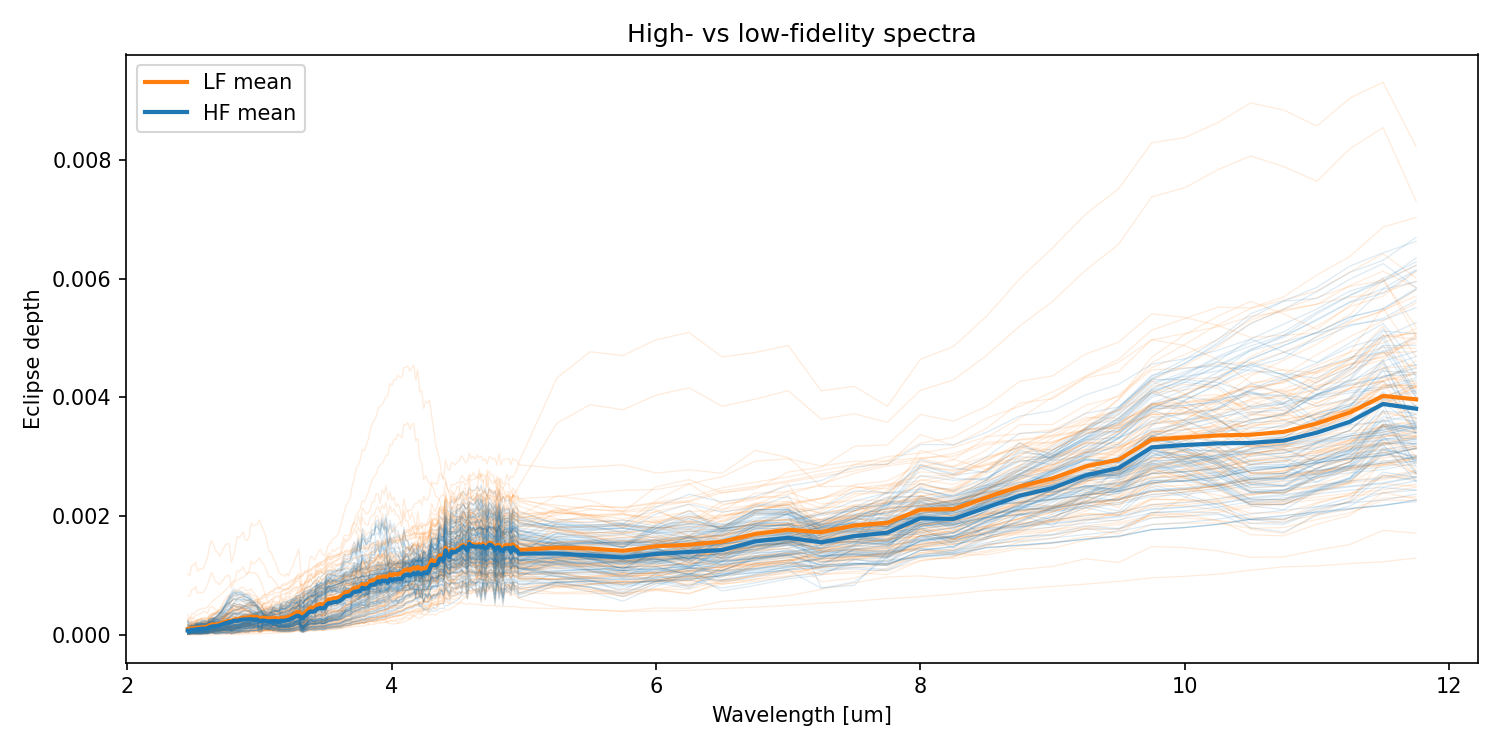
\includegraphics[width=0.90\linewidth]{figures/00_hf_vs_lf.png}
  \caption{HF training spectra (individual samples) and the $\nLFtenk{}$-point LF
  design summarised by its $5$--$95\%$ band across wavelength.}
  \label{fig:hf_vs_lf}
\end{figure}

\begin{figure}[h]
  \centering
  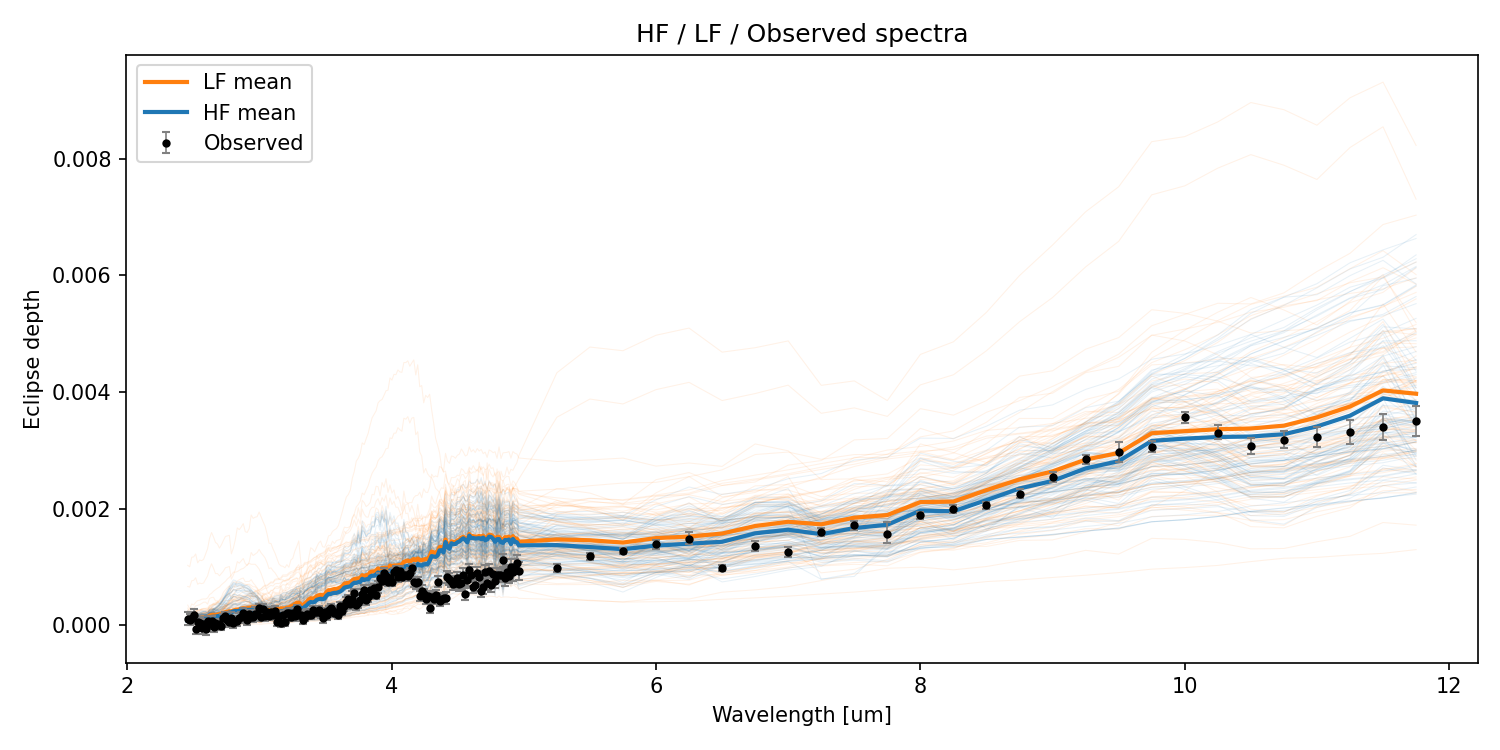
\includegraphics[width=0.90\linewidth]{figures/00_hf_lf_observed.png}
  \caption{HF training spectra and the $\nLFtenk{}$-point LF design
  ($5$--$95\%$ band), overlaid on the observed spectrum of
  WASP-80b with error bars (black).}
  \label{fig:hf_lf_observed}
\end{figure}

\begin{figure}[h]
  \centering
  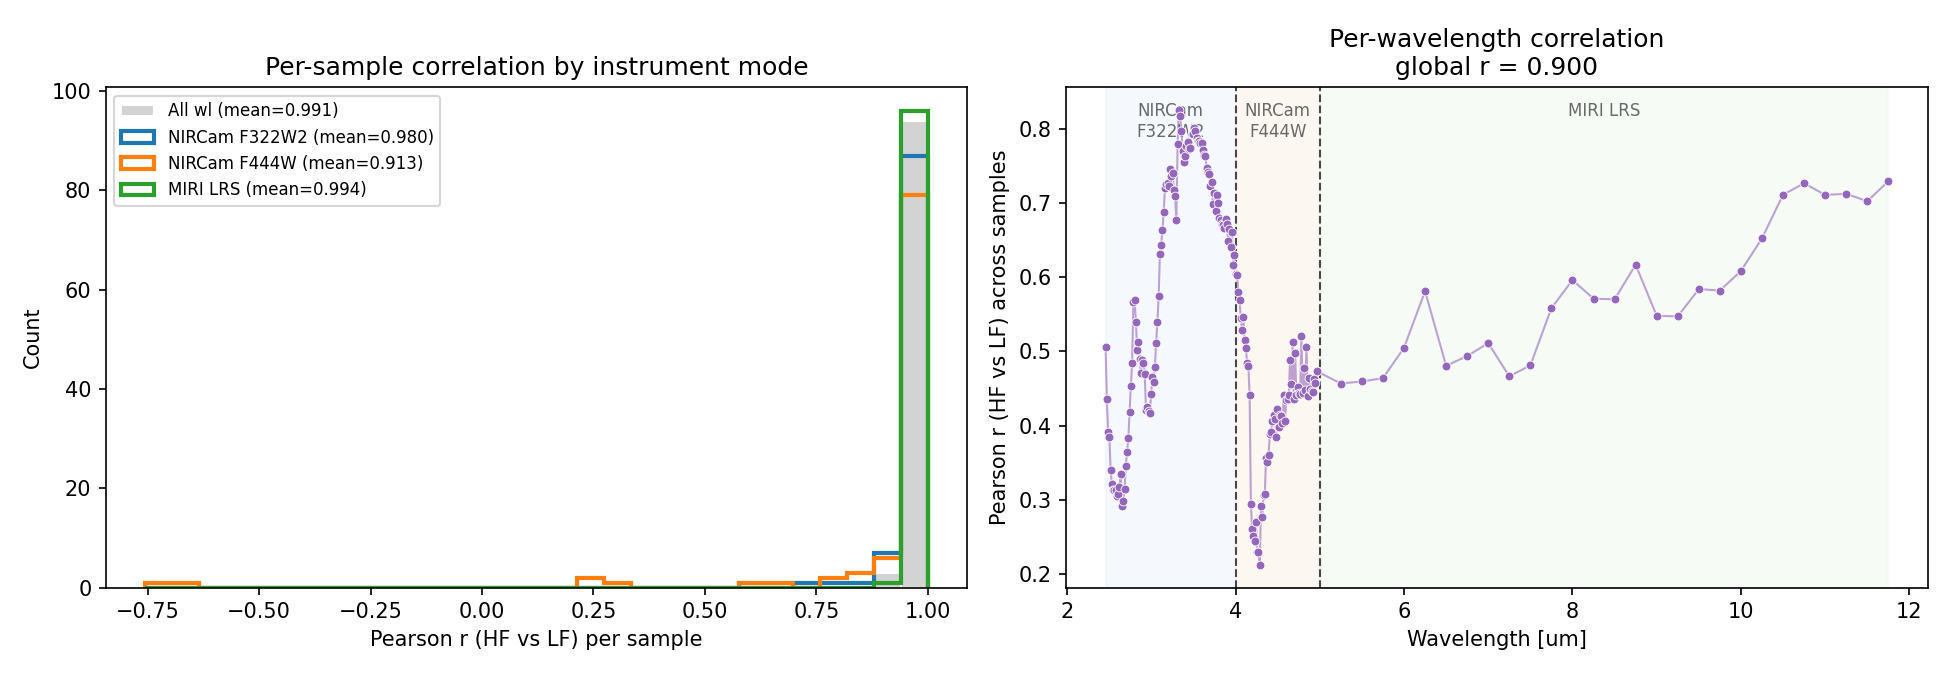
\includegraphics[width=0.95\linewidth]{figures/00_hf_lf_correlation.png}
  \caption{Pearson correlations between $Y^{HF}$ and $Y^{LF}$ (paired LF).
  \emph{Left:} per-sample correlations computed across wavelength at each design
  point, split into the three instrument modes (NIRCam~F322W2,
  NIRCam~F444W, and MIRI~LRS). \emph{Right:}
  per-wavelength correlation $r_{\lambda}^{(j)}$ across the $\nHF{}$
  design points as a function of $\lambda_{j}$, with the minimum
  $r_{\lambda}=\perwlmin{}$ at the CO$_2$ band near $\perwlminlam\,\mu$m.}
  \label{fig:correlation}
\end{figure}

The geometry behind these correlations is shown in Figure~\ref{fig:oblique_hflf}:
viewing the training set as one HF--LF cloud per wavelength makes the per-bin slope
$\rho_j$ directly visible as the tilt of each slice, while the structured collapse of
$r^{(j)}_\lambda$ across $4.0$--$4.7\,\mu$m appears as a band of slices that
simultaneously flatten (small $\rho_j$) and broaden (large unexplained scatter). This
is precisely the regime a per-bin multifidelity coupling is designed to exploit, and
it motivates letting $\rho_j$ vary across bins in Model~1 (Section~\ref{subsec:model1}).

\paragraph{What $\rho_j$ is, and how it is computed.}
Each coloured slice in Figure~\ref{fig:oblique_hflf} is a single wavelength bin
$\lambda_j$, and its colour is the \emph{per-bin slope} $\rho_j$ --- the same
scalar that couples the two fidelities in Model~1,
$f_{H,j}=\rho_j f_{L,j}+\delta_j$ (Section~\ref{subsec:model1}). It is obtained
bin-by-bin, not from any joint fit. For a fixed bin $j$ we take the $\nHF{}$
co-located HF/LF pairs $\{(y^{L}_{i,j},\,y^{H}_{i,j})\}_{i=1}^{\nHF}$ (the HF
design nested in the LF set, Eq.~\ref{eq:design_nested}), centre each fidelity by
its across-sample mean $\bar y^{L}_{j},\bar y^{H}_{j}$, and define $\rho_j$ as the
ordinary least-squares slope of the centred HF residual regressed on the centred
LF residual:
\begin{equation}
  \rho_j
  \;=\;
  \frac{\sum_{i=1}^{\nHF}\bigl(y^{H}_{i,j}-\bar y^{H}_{j}\bigr)
        \bigl(y^{L}_{i,j}-\bar y^{L}_{j}\bigr)}
       {\sum_{i=1}^{\nHF}\bigl(y^{L}_{i,j}-\bar y^{L}_{j}\bigr)^{2}}
  \;=\;
  \frac{\operatorname{Cov}_i\!\bigl(y^{H}_{\cdot,j},\,y^{L}_{\cdot,j}\bigr)}
       {\operatorname{Var}_i\!\bigl(y^{L}_{\cdot,j}\bigr)}
  \;=\;
  r_{\lambda}^{(j)}\,\frac{s_{H,j}}{s_{L,j}},
  \label{eq:rho-per-bin}
\end{equation}
where $s_{H,j},s_{L,j}$ are the across-sample HF and LF standard deviations at
bin $j$ and $r_{\lambda}^{(j)}$ is the per-wavelength correlation defined above.
Under the AR(1) multi-fidelity model this OLS value is exactly the
maximum-likelihood estimate of the scaling factor when the discrepancy is
directly observable, so the recursive scheme of Model~1 simply reads $\rho_j$ off
\eqref{eq:rho-per-bin} before fitting $\delta_j$ to the residuals. In the figure
both residuals are divided by the \emph{same} factor $s_{L,j}$, which fixes the
horizontal (LF) spread to unity in every bin and leaves the slope unchanged; the
visible tilt of each slice is therefore $\rho_j$ itself.

\paragraph{Why $\rho_j$ varies, and what it means.}
The decomposition $\rho_j=r_{\lambda}^{(j)}\,(s_{H,j}/s_{L,j})$ in
\eqref{eq:rho-per-bin} splits the slope into two multiplicative effects: how well
the fidelities co-vary ($r_{\lambda}^{(j)}$) and how much HF dynamic range remains
relative to LF ($s_{H,j}/s_{L,j}$). Both shrink inside the $4.3\,\mu$m CO$_2$
band: the ranking of samples decorrelates ($r_{\lambda}$ falls to $\perwlmin{}$)
\emph{and} HF saturation compresses $s_{H,j}$ by ${\sim}40\%$ while $s_{L,j}$ is
unchanged. The two factors compound, which is why $\rho_j$ collapses to the dark
($\rho_j\!\approx\!0.2$) slices there and rises to the bright
($\rho_j\!\approx\!0.5$--$0.65$) slices in the continuum. Note that $\rho_j<1$
everywhere: in standardised units a unit LF excursion maps to a sub-unit HF
excursion, i.e.\ the LF systematically over-disperses relative to the HF. Where
$\rho_j$ is smallest the scaled LF term $\rho_j y^{L}$ explains least, so almost
all of the HF structure must be carried by the discrepancy $\delta_j$ --- and that
is precisely the band where $\delta_j$ also shows the largest unexplained
scatter, making it the hardest region for any multi-fidelity surrogate and the
clearest motivation for letting the coupling vary with wavelength.

\begin{figure}
  \centering
  \includegraphics[width=\textwidth]{figures/oblique_view_training_data.png}
  \caption{Oblique view of the per-wavelength MFGP training data on the WASP-80b design ($n=97$ inputs, $m=195$ wavelength bins). Each wavelength $\lambda_j$ defines a slice containing its $97$ high-/low-fidelity training pairs $(y^{L}_{i,j},\,y^{H}_{i,j})$, standardised per bin by removing the bin means and dividing \emph{both} residuals by the low-fidelity standard deviation $s_{L,j}$; the horizontal spread is therefore unit in every bin and the tilt of a slice equals the per-bin slope $\rho_j$. The straight line in each slice is the bin-wise regression, coloured by $\rho_j$. \emph{Left:} a general oblique angle.
    \emph{Right:} the same data viewed down the $\lambda$-axis.}
  \label{fig:oblique_hflf}
\end{figure}

\subsection{Instrument structure and its modelling implications}
\label{subsec:instrument-structure}

The observed spectrum of WASP-80b combines three distinct JWST instrument
modes: NIRCam~F322W2 and
NIRCam~F444W on the short-wavelength side, and MIRI~LRS on the
long-wavelength side. Their observing configurations and noise characteristics
differ, while the NIRCam-to-MIRI transition also changes spectral resolution
and imposes the structural break in the wavelength grid
noted in Section~\ref{sec:what}: $103$ NIRCam~F322W2 bins in the nominal
$2.4$--$4\,\mu$m band, $65$ NIRCam~F444W bins in the $4$--$5\,\mu$m band,
and $27$ MIRI~LRS bins in the $5$--$12\,\mu$m band. The NIRCam bins have
width $\Delta\lambda=0.015\,\mu$m, while the sampled MIRI~LRS bins have
width $\Delta\lambda=0.25\,\mu$m and begin at $5.25\,\mu$m. Because the
HF--LF agreement reported above has different mode-level summaries, the
instrument boundaries are a natural axis along which to organise the
surrogate; the strong variation within the NIRCam modes must still be modelled
as wavelength-dependent structure.

This suggests two complementary ways of accommodating the instrument
structure. The first is to absorb it into the scaling factor: rather than a
single global $\rho$, one lets $\rho=\rho(\lambda)$ vary across wavelength
(Section~\ref{subsec:correlation-modelling}), so that the differing HF--LF
agreement of the three instrument modes is captured by one model with a
wavelength-dependent correlation, possibly with mode-specific length-scales or
a piecewise wavelength kernel at the $4$ and $5\,\mu$m mode boundaries (the
latter also being a grid-resolution break). The
second is to partition the problem by instrument and fit three separate
multi-fidelity models, one for each mode (NIRCam~F322W2, NIRCam~F444W,
MIRI~LRS), each with its own scaling, kernels, and noise variances, and then
concatenate their predictions across the full grid. Fitting per instrument
removes the need to bridge the resolution and noise discontinuity inside a
single kernel and lets each mode's HF--LF relationship be estimated on its
own terms, at the cost of not sharing statistical strength across the
boundaries and of estimating each model from a smaller wavelength range.

%==========================================================================
\section{Bayesian Inversion Framework}
\label{sec:bayesian-inversion}
%==========================================================================
\textcolor{red}{The Bayesian inversion is part of the larger project scope, whether it
sits inside the semester paper or outside.
The section is kept here as a placeholder so that the surrogate construction in \S\ref{sec:gpmf} is designed with the downstream likelihood in mind.}

% \researchq{Once a surrogate exists, how is it embedded into the posterior, and
% which assumptions in the thesis pipeline are worth revisiting?}

\subsection{Likelihood model}
\label{sec:likelihood}
The likelihood is Gaussian with diagonal covariance,
\[
\mathcal{L}(\yv_{\mathrm{obs}} \mid \theta) \;=\;
\prod_{j=1}^{m}
\mathcal{N}\!\bigl(y_{\mathrm{obs},j}\,\big\vert\,
M_{j}(\theta),\;
\sigma^{2}_{\mathrm{tot},j}\bigr),
\qquad
\sigma^{2}_{\mathrm{tot},j} \;=\;
\sigma^{2}_{\mathrm{obs},j} + \sigma^{2}_{\mathrm{surrogate},j},
\]
with $M_{j}(\theta) = \hat y^{SF}_{j}(\theta)$ the surrogate prediction
at the $j$-th wavelength and $\sigma^{2}_{\mathrm{surrogate},j}$ the
diagonally propagated LOO variance. The diagonal structure assumes
independence of the residuals across wavelength bins, both
observationally and at the surrogate level.

\subsection{Priors and the design-domain identity}
The priors $\pi(\theta)$ are identical to the LHS design domain of
Table \ref{tab:inputs}, with $\Rp$ and $\logg$ given narrow Gaussian priors centred
on the literature values for WASP-80b. The posterior support therefore coincides with the surrogate's training support. 



\subsection{Sampling and convergence diagnostics}
Posterior sampling uses Adaptive Metropolis with $600$ chains $\times$ $40\,000$ iterations and a
$60\%$ burn-in. 

% %==========================================================================
% \section{Open Questions and Project Hooks}
% %==========================================================================
% \researchq{What remains genuinely unclear after a careful reading, and which of
% those gaps does our project intend to close?}

% \subsection{Unclear in the thesis}
% \begin{itemize}[leftmargin=2em,itemsep=0.2em]
%   \item \emph{UQLab implementation of the intermediate profile
%         surrogates.} The thesis states that ``independent PCE
%         surrogates are trained'' for the pT profile and for each of the
%         six abundance profiles, but does not make explicit whether each
%         retained PC is a separate scalar-output PCE or whether UQLab is
%         silently fitting a joint multivariate-output model.
%   \item \emph{Total retained PCs across intermediate surrogates.} The
%         informally circulated ``${\sim}40$'' figure is plausible as a
%         sum $q_{T} + \sum_{m\in\mathcal{M}} q_{m}$ across the seven
%         intermediate response blocks, but the thesis never lists a
%         breakdown.
%   \item \emph{Treatment of the $5\,\mu$m grid break.} The wavelength
%         grid contains a structural discontinuity between $4.96\,\mu$m
%         (NIRCam F444W) and $5.25\,\mu$m (MIRI LRS), with a
%         factor-${\sim}17$ jump in bin width. The thesis does not state
%         whether the noise model or surrogate-variance estimate treats
%         all three instrument modes separately or pools them.
%   \item \emph{Asymmetric observational error bars.} The published
%         WASP-80b spectrum reports
%         $\mathtt{measured\_err\_lo}$ and $\mathtt{measured\_err\_hi}$
%         as distinct columns, but the diagonal Gaussian likelihood used
%         in the inversion takes one $\sigma_{\mathrm{obs},j}$ per bin.
%         The thesis does not document how (or whether) these were
%         symmetrised.
%   \item \emph{Why MF fails at the level of the leading PCs.} The thesis
%         attributes the failure to ``noise'' in the discrepancy scores
%         but does not separate the three candidate causes (chemistry
%         truncation, PCA truncation of intermediate profiles, PCE
%         smoothing).
% \end{itemize}

% \subsection{What our project will resolve}
% Mapped to the proposed work plan: (i)~reproducing the SF baseline in
% Python under matched priors pins down the UQLab implementation
% ambiguity (open question 1 above) and produces the breakdown of
% retained PCs across intermediate surrogates (open question 2);
% (ii)~replacing PCE by a per-PC GP and by an LMC multi-output GP probes
% whether the polynomial smoothing of PCE drives the carbon bias and
% provides the right machinery to model the $5\,\mu$m grid break as a
% piecewise kernel (open question 3); (iii)~the one-step AR(1) GP MF
% model of \S\ref{sec:gpmf}, applied to the same LF / HF training pairs,
% gives a direct probe of whether the leading-PC discrepancy failure is
% due to data sparsity or to the rigidity of PCE (open question 5); and
% (iv)~the observed spectrum will be loaded with both
% $\mathtt{measured\_err\_lo}$ and $\mathtt{measured\_err\_hi}$
% preserved, and the symmetrisation choice will be made explicitly and
% documented (open question 4).

%==========================================================================
% \section*{References}
% \addcontentsline{toc}{section}{References}
% %==========================================================================

% \begin{description}[leftmargin=1.2em,itemsep=0.3em]
% \item Rasmussen \& Williams (2006), \emph{Gaussian Processes for Machine
%   Learning}, MIT Press. Free PDF at
%   \url{http://www.gaussianprocess.org/gpml/}. 
% \item Peherstorfer, Willcox \& Gunzburger (2018),
%   \emph{SIAM Review} 60(3), 550--591 
% \item Kennedy \& O'Hagan (2000), \emph{Biometrika} 87(1) for the original
%   autoregressive model and Le Gratiet \& Garnier (2014) for the
%   recursive form most software actually implements.
% \item[PCE:]
%   Sudret (2008), \emph{Reliab.~Eng.~Syst.~Saf.}~93(7) and Blatman \&
%   Sudret (2011), \emph{J.~Comput.~Phys.}~230. Both are short and
%   algorithmic.
% \item[Atmospheric retrieval:]
%   Madhusudhan (2018), in \emph{Handbook of Exoplanets}, Springer ---
%   the broad review to skim.
%   Mollière et al.~(2019), A\&A 627, A67 --- petitRADTRANS itself.
% \item[Bayesian computation:]
%   Goodman \& Weare (2010), \emph{Comm.~Appl.~Math.~Comput.~Sci.}~5(1)
%   for AIES; Vehtari et al.~(2021), \emph{Bayesian Analysis} 16(2) for
%   diagnostics. Use Gelman et al., \emph{BDA3}, only as a reference.
% \end{description}


%==========================================================================
\appendix
%==========================================================================
\section{Previous Methodology (Céline's pipeline)}
%==========================================================================

\noindent The methodology summarised in this appendix is the prior pipeline of Céline, retained here as background and as the baseline against which the multi-fidelity GP methodology of Section~\ref{sec:gpmf} is compared. It used a co-located $97/97$ HF/LF design, in contrast to the enlarged LF design ($N_L=10\,000$, $\bm{X}_H\subset\bm{X}_L$) adopted in the main text.
The four subsections below summarise Céline's pipeline, which serves as the previous methodology against which the proposed approach will be compared. In her work, at a high level, the modelling hierarchy proceeds from an expensive physical simulator to training-data generation, surrogate fitting, and finally Bayesian retrieval:
\[
\text{physical simulator}
\;\longrightarrow\;
\text{training data}
\;\longrightarrow\;
\text{surrogate fitting}
\;\longrightarrow\;
\text{Bayesian retrieval}.
\]
Figure~\ref{fig:celine-model-hierarchy} makes this hierarchy explicit by separating
the HF simulator outputs, the fitted SF/LF/MF surrogate components, and their use
inside the Bayesian inversion.

\begin{center}
    \begin{figure}
    \centering
    \includegraphics[width=0.75\linewidth]{figures/Celine's.png}
    \caption{Model hierarchy from HF simulations to SF/MF spectral predictions and Bayesian inversion of atmospheric parameters. Colors distinguish the main blocks: inputs, HF simulator outputs, training data, surrogate fitting, LF prediction, MF correction, and Bayesian inversion.}
    \label{fig:celine-model-hierarchy}
\end{figure}
\end{center}



\textcolor{red}{For the scope of our work, one could ideally ignore the physical nature that makes one high and one low in fidelity. I found it clarifying to go through the methodology for it anyway. The most important thing to point out, is that while the model changes, the input design matrix for both fidelities was the same.}\\

\subsection{The High-Fidelity Forward Model}
A single HF computation is the iterated application of four physical
modules, taking the $9$-vector $\xv$ as input and returning the
spectrum $\yhf(\xv)$:
\[
\xv \;\xrightarrow{\text{FastChem}}\; \{X_{m}^{\,\mathrm{eq}}(p)\}
\;\xrightarrow{\text{HELIOS-K}}\; \{\kappa_{m}(\lambda,p,T)\}
\;\xrightarrow{\text{HELIOS}}\; T(p)
\;\xrightarrow{\text{VULCAN}}\; \{X_{m}(p)\}
\;\xrightarrow{\text{petitRADTRANS}}\; \yhf(\xv).
\]
\emph{FastChem} computes equilibrium chemical abundances on the
vertical pressure grid given elemental ratios and a temperature
profile. \emph{HELIOS-K} produces the molecular line opacities
$\kappa_{m}$ on the wavelength/pressure/temperature grid. \emph{HELIOS}
is the $1$D radiative--convective equilibrium solver that computes the
temperature profile $T(p)$ from the opacities, the stellar irradiation,
and the heat-redistribution factor $\fhr$. \emph{VULCAN} relaxes
equilibrium chemistry to a disequilibrium steady state under vertical
mixing (parameterised by $K_{zz}$) and photochemistry. Finally,
\emph{petitRADTRANS} performs the line-by-line radiative transfer on
the converged $(T(p),X_{m}(p))$ state and returns the spectrum.
\litref{Mollière et al.~(2019), ``petitRADTRANS,'' A\&A 627, A67.}

The chain is iterated because the chemistry depends on $T(p)$ and the
temperature profile depends, through opacities, on the abundances. One
outer step reads
\[
T^{(t)}(p) \;\longrightarrow\; \{X_{m}^{(t+1)}(p)\}
\;\longrightarrow\; T^{(t+1)}(p),
\]
and iteration stops when $\|T^{(t+1)}-T^{(t)}\|$ falls below a fixed
tolerance. The loop guarantees mutual consistency of thermal structure
and chemistry; it does not guarantee uniqueness of the converged
state.


The high-fidelity simulator maps atmospheric input parameters to spectra:
\[
f_{\mathrm{HF}}:\mathcal X\subset\mathbb R^9\to\mathbb R^{195},
\qquad
x\mapsto y_{\mathrm{HF}}(x).
\]


\subsubsection{Computational cost and the design of experiments}
A single HF evaluation costs hours to a day. The training set is fixed
at $n = 97$ design points produced by Latin-hypercube sampling (LHS) on
$\mathcal{X}$. LHS guarantees that each one-dimensional marginal is
stratified into $n$ equal-probability bins (one point per stratum),
which prevents the worst-case clustering of i.i.d.\ sampling. The
dominant limitation, which propagates through everything that follows,
is sparsity: $97$ points in $\mathbb{R}^{9}$ correspond to a mean
nearest-neighbour spacing that is large relative to the characteristic
length scales of the spectral response.\\
% \thref{Section 3.\ldots\ on training data generation; Table~3.1 for the
% design domain.}\\
% \litref{Forrester, Sobester \& Keane (2008), \emph{Engineering Design
% via Surrogate Modelling} --- Chapter 1 covers LHS and design quality
% metrics in a very accessible way.}

\subsection{The Low-Fidelity Forward Model}
The LF retrieval is evaluated on exactly the same input design
matrix as the HF retrieval: the same $97$ LHS points
$\{\xv^{(i)}\}_{i=1}^{97}$. 
% This is important for the multi-fidelity  construction --- it means the discrepancy
% $\delta(\xv^{(i)}) = \yhf(\xv^{(i)}) - \rho\,\ylf(\xv^{(i)})$ is
% available pointwise on the training design and can be regressed on
% $\xv$ without any further design choice.

The LF reduction consists in dropping the expensive self-consistency loop. Instead of solving the coupled chemistry/thermal-structure problem for each $\xv$, ``cheap'' regression maps 
\[
\xv \;\longmapsto\; \hat T(\cdot;\xv), \qquad
\xv \;\longmapsto\; \{\hat X_{m}(\cdot;\xv)\}_{m\in\mathcal{M}}
\]
return surrogate (see details in Section ~\ref{sec:pcapck}) pressure--temperature and abundance profiles, which
are then passed into petitRADTRANS to obtain the LF emission spectrum
$\ylf(\xv)$. The LF model is a surrogate-driven object that re-uses part of the HF physical emulator (petitRADTRANS) but bypasses
the iterated $(T,\{X_{m}\})$ coupling, with three associated structural
biases (chemistry truncation to $\mathcal{M}$, PCA truncation of the
profile responses, PCE smoothing of the score regressions).
Specifically, the stages to build the LF data are:
\begin{enumerate}[leftmargin=2em,itemsep=0.2em]
  \item For each retained PC of the centred matrix of pT profiles
        $\tilde Y^{T}$ across the training design, fit an independent
        PCE $\hat\alpha^{T}_{k}(\xv)$, and reconstruct
        \[
        \hat T(p;\xv) \;=\; \bar T(p) + \sum_{k=1}^{q_{T}}
        \hat\alpha^{T}_{k}(\xv)\,V^{T}_{k}(p).
        \]
  \item For each species $m \in \mathcal{M}$ and each retained PC of
        its centred abundance matrix $\tilde Y^{X_{m}}$, fit an
        independent PCE $\hat\alpha^{X_{m}}_{k}(\xv)$, and reconstruct
        \[
        \hat X_{m}(p;\xv) \;=\; \bar X_{m}(p) + \sum_{k=1}^{q_{m}}
        \hat\alpha^{X_{m}}_{k}(\xv)\,V^{X_{m}}_{k}(p).
        \]
  \item Pass the reconstructed atmospheric state into petitRADTRANS:
        \[
        \ylf(\xv) \;=\;
        \mathrm{petitRADTRANS}\!\bigl(\hat T(\cdot;\xv),
        \{\hat X_{m}(\cdot;\xv)\}\bigr)
        \;\in\; \mathbb{R}^{m}.
        \]
\end{enumerate}
Schematically,
\[
\xv \;\xrightarrow{\text{PCE}_{T},\,\text{PCE}_{X_{m}}}\;
\bigl(\hat T(\cdot;\xv),\,\{\hat X_{m}(\cdot;\xv)\}\bigr)
\;\xrightarrow{\text{petitRADTRANS}}\; \ylf(\xv).
\]
% This is the ``two-step'' (more precisely, three-stage) construction
% the supervisor refers to.\\
% \thref{Section 4.4.1 (pp.~30--32); schematic figures in Appendix A.}

\subsection{Surrogate Modelling}

%\textcolor{red}{The term "surrogate" is at times abused both in Celine's and in this note.}

\subsubsection{The Single-Fidelity (SF) Surrogate}

The SF surrogate provides the baseline statistical emulator of the HF forward map.
It treats the available HF simulations as the sole training source and learns an in-sample approximation of
\[
x \longmapsto y_{\mathrm{HF}}(x).
\]
In this sense, the SF surrogate directly replaces the expensive HF simulator by a
cheap statistical map from atmospheric parameters to spectra. No use of other lower fidelities is done, and the difference with the LF model is that SF is purely statistical and no petitRADTRANS is needed.

\paragraph{PCA on the spectral output.}
Build the response matrix using the $n=97$ HF training spectra as rows of
$Y^{HF}\in\mathbb{R}^{n\times m}$ and centre by the training mean
$\bar{\yv}^{HF} = \tfrac{1}{n}\sum_{i}\yhf(\xv^{(i)})$. Truncated SVD
of the centred matrix $\tilde Y^{HF}$ gives an orthonormal basis
$V_{K} \in \mathbb{R}^{m\times K}$ and PC scores
$A_{K}\in\mathbb{R}^{n\times K}$, so that
\[
\yhf(\xv^{(i)}) \;=\; \bar{\yv}^{HF}
\;+\; \sum_{k=1}^{K} z_{k}^{(i)}\,\bm{\phi}_{k}
\;+\; \varepsilon^{(i)},
\qquad z_{k}^{(i)} = (A_{K})_{i,k},\quad
\bm{\phi}_{k} = V_{K}^{(\cdot,k)},
\]
with $\varepsilon^{(i)}$ the PCA-truncation residual. The number of
retained components is chosen by an LOO-based rule: a PC $k$ is kept
only if the normalised LOO error of its score-level surrogate clears
\[
\frac{\sigma^{2}_{\mathrm{surrogate},k}}
     {\sigma^{2}_{\mathrm{data},k}} \;<\; 0.8 .
\]
For the final HF spectrum this leaves $K = 5$. The threshold is an
emulator-side criterion and is not tied to any downstream loss
(e.g.\ retrieval bias on $\XC$).
So, all further modelling, will try and build a surrogate for this subset mapping instead of (\ref{eq:ammotelodico}):
\[
\hat{f}:\mathbb{R}^9\longrightarrow\mathbb{R}^{K},\;\; K=5
\].


% \thref{Section 4.3 (PCA setup); threshold discussion.}\\
% \litref{Jolliffe \& Cadima (2016), ``Principal component analysis: a
% review and recent developments,'' \emph{Phil.~Trans.~R.~Soc.~A}.}

\paragraph{Polynomial chaos expansion on the PC scores.}
\label{sec:pcapck}
For each retained PC index \(k=1,\dots,K\), the scalar map from
atmospheric parameters to the corresponding PC score is approximated
statistically. Polynomial chaos expansion (PCE) represents this map as a
global expansion in multivariate orthonormal polynomials of the input
variables:
\[
z_k(\xv)
\approx
\hat z_{k}(\xv)
=
\sum_{\bm{\alpha}\in\mathcal{A}_{k}}
c_{k,\bm{\alpha}}\,
\Psi_{\bm{\alpha}}(\xv), \; \bm{\alpha}=(\alpha_1,\dots,\alpha_d)\
\]
Here
\(\Psi_{\bm{\alpha}}\) denotes a tensorised polynomial basis function,
and \(c_{k,\bm{\alpha}}\) are regression coefficients estimated from
the training data. The basis is chosen to be orthonormal with respect to
the input distribution. PCE provides a
smooth global regression model for each retained PC score, rather than
an interpolating fit through all training points. The truncation set
\(\mathcal{A}_{k}\), which determines which polynomial
degrees are retained, is selected adaptively by sparse regression following Blatman and Sudret (2011).

As an alternative, \textbf{polynomial chaos--kriging} (PCK) was also considered.
PCK combines a PCE trend with a Gaussian-process residual correction:
\[
z_k(\xv)
=
\sum_{\bm{\alpha}\in\mathcal{A}_{k}}
c_{k,\bm{\alpha}}\,
\Psi_{\bm{\alpha}}(\xv)
+
Z_k(\xv),
\]
where \(Z_k(\xv)\) is a zero-mean Gaussian process with covariance
kernel
\[
\mathrm{Cov}\!\left(Z_k(\xv),Z_k(\xv')\right)
=
\sigma_k^2 R_k(\xv,\xv').
\]
The PCE component captures the global polynomial trend, while the
Kriging component models local residual deviations.
This makes PCK more flexible than pure PCE, but also more prone to
interpolation artefacts when the training set is small and the target
scores contain noise induced by PCA truncation.


\paragraph{Reconstruction of the full spectrum.}
The full spectrum is reconstructed by inverse PCA:
\[
\hat{\yv}^{SF}(\xv) \;=\; \bar{\yv}^{HF}
\;+\; \sum_{k=1}^{K} \hat z_{k}(\xv)\,\bm{\phi}_{k}
\;=\; \bar{\yv}^{HF} + V_{K}\,\hat{\bm z}(\xv).
\]
The surrogate's per-bin variance is approximated by propagating the LOO residual
variance of the score-level PCEs through the linear inverse PCA map:
\[
\sigma^{2}_{\mathrm{surr},j}
=
\sum_{k=1}^{K} V_{K,jk}^{2}\,\sigma^{2}_{\mathrm{LOO},k}.
\]
% This corresponds to assuming that the surrogate prediction errors of the retained
% PC scores are uncorrelated and that their variances are constant over the input
% space. A more complete propagation would use the full empirical covariance matrix
% of the LOO score residuals,
% \[
% \Sigma_{\mathrm{surr}}
% =
% V_K
% \Sigma_{z,\mathrm{LOO}}
% V_K^\top,
% \]
% thereby retaining cross-PC error covariance and the induced wavelength-to-wavelength
% correlations.

\subsubsection{The Multi-Fidelity (MF) Construction --- Two-Step Pipeline}
% \researchq{What does Céline's MF model actually compute, and where do the LF
% and HF input spaces fail to coincide?}
The MF modelling used represents HF data as a scaled LF plus a discrepancy term,
\[
\yhf(\xv) \;\approx\; \rho\,\ylf(\xv) \;+\; \delta(\xv),
\]
with $\rho \in \mathbb{R}$ a scalar correlation/scaling factor and $\delta\colon\mathcal{X}\to\mathbb{R}^{m}$ the learned discrepancy. 

%  A log-space variant may also be implemented:
% \[
% \log\yhf(\xv) \;\approx\; \tilde\rho\,\log\ylf(\xv)
% \;+\; \tilde\delta(\xv)
% \].
% \\
% \thref{Eq.~(3.1) on p.~13; Eqs.~(4.3)--(4.6) on pp.~32--33.}\\
% \litref{Kennedy \& O'Hagan (2000), \emph{Biometrika} 87(1) --- the
% original paper.}\\
% \litref{Peherstorfer, Willcox \& Gunzburger (2018), ``Survey of
% multifidelity methods,'' \emph{SIAM Review} 60(3) --- the modern
% standard survey, and the one to cite when motivating the GP MF
% alternative.}

\paragraph{The discrepancy surrogate}
Once $\ylf(\xv^{(i)})$ is available at every training point, the additive discrepancy is computed in the shared spectral space,
\[
\delta(\xv^{(i)}) \;=\; \yhf(\xv^{(i)}) - \rho\,\ylf(\xv^{(i)}),
\qquad i = 1,\dots,n,
\]
with $\rho$ fitted as a scalar from the training pair. PCA is applied
to the centred discrepancy matrix $\tilde\Delta\in\mathbb{R}^{n\times m}$,
yielding basis $V^{\delta}$ and scores $\alpha^{\delta}_{k}$; one PCE
is fitted per retained discrepancy PC,
\[
\hat\alpha^{\delta}_{k}(\xv) \;=\;
\sum_{\bm{\alpha}\in\mathcal{A}^{\delta}_{k}}
c^{\delta}_{k,\bm{\alpha}}\,\Psi_{\bm{\alpha}}(\xv),
\qquad
\hat{\ymf}(\xv) \;=\; \rho\,\ylf(\xv)
\;+\; \underbrace{V^{\delta}\,\hat{\bm\alpha}^{\delta}(\xv)}_{=\hat\delta(\xv)}.
\]
% Under the same LOO threshold $0.8$, only the \emph{ninth} discrepancy
% PC clears the bar (Fig.~4.10); the leading discrepancy PCs --- which
% carry most of the structural LF--HF gap --- are too noisy to surrogate
% from $97$ training points. The MF correction therefore lacks the
% dominant structural information and underperforms the SF model across
% the wavelength range (Fig.~4.11), which is why MF is not plugged into
% the Bayesian inversion.\\
% \thref{Section 4.4.2 (pp.~32--34); Fig.~4.10, Fig.~4.11.}

% \paragraph{Why we call this ``two-step''}
% A textbook one-step MF emulator fits a single joint statistical model
% that ties LF and HF together in the same output space (typically by a
% co-kriging or autoregressive GP, \S\ref{sec:gpmf}). Nussbaumer's MF is
% instead a \emph{composition} of three surrogate stages
% ($\xv\to\hat T,\hat X_{m}$; $\hat T,\hat X_{m}\to\ylf$;
% $\xv\to\hat\delta$) wrapped around one physical solver
% (petitRADTRANS). The LF/HF input-space mismatch ---
% petitRADTRANS does not consume $\xv$ directly, but the atmospheric
% state $(T,\{X_{m}\})$ --- is reconciled \emph{by surrogate composition}
% from the common $9$-vector into the state variables; it is \emph{not}
% reconciled by the choice of statistical model.

% \subsection{Limitations and Needed Improvements}
% The limitations of the previous methodology that motivate the GP
% alternative below cluster into four points.
% First, the diagonal $\Sigma_{\mathrm{surr}}$ and the diagonal
% $\Sigma_{\mathrm{obs}}$ in the likelihood are inconsistent with the
% construction of the surrogate (a linear combination of $K$ smooth
% basis functions induces wavelength-correlated errors by design) and
% with JWST instrumental systematics.
% Second, the hard PC-keep / PC-drop threshold at $0.8$ is an
% emulator-only rule decoupled from retrieval-level loss; in particular,
% it discards every leading discrepancy PC in the MF model.
% Third, PCE is a polynomial smoother that washes out narrow chemically
% informative features in higher PCs; this is the most plausible
% explanation for the systematic carbon underestimation reported in
% Chapter 6 (the narrow CO / CO$_{2}$ / CH$_{4}$ features sit precisely
% in the high-frequency content the higher PCs would resolve).
% Fourth, the MCMC reporting omits split-$\hat R$, bulk/tail-ESS,
% integrated autocorrelation time, and per-chain acceptance rates ---
% precisely the diagnostics one needs in the multimodal /
% bound-piled regime the thesis itself discusses.

\subsection{Validation of the HF spectral prediction}

Validation focuses on whether the surrogate accurately predicts the
high-fidelity spectrum
\[
y_{\mathrm{HF}}(x)\in\mathbb R^{195}
\]
at unseen atmospheric input points. Since the HF output is high-dimensional,
validation is carried out after PCA compression of the spectra. The HF
response matrix
\[
Y^{\mathrm{HF}}\in\mathbb R^{97\times 195}
\]
is decomposed into principal components, and scalar surrogates are fitted to
the retained PC scores. In the final SF spectral surrogate, the first five
spectral principal components are retained. 

For each retained PC score \(z_k(x)\), the surrogate is validated using
leave-one-out cross-validation. The full HF spectrum is then reconstructed
by inverse PCA:
\[
\hat y_{\mathrm{SF}}(x)
=
\bar y^{\mathrm{HF}}
+
V_K \hat z(x),
\]
where \(V_K\in\mathbb R^{195\times K}\) contains the retained spectral PC
basis vectors. The spectral prediction is then validated by comparing the
LOO-reconstructed spectra
\[
\hat y_{\mathrm{SF}}^{(-i)}(x_i)
\]
against the corresponding HF spectra, or more precisely against their
PCA-smoothed reconstructions
\[
y_i^{\mathrm{rec}}
=
\bar y^{\mathrm{HF}}
+
V_KV_K^\top
\left(y_i^{\mathrm{HF}}-\bar y^{\mathrm{HF}}\right).
\]

The same LOO residuals are used to estimate the wavelength-dependent
surrogate variance:
\[
\sigma^2_{\mathrm{surr},j}
=
\frac{1}{n}
\sum_{i=1}^{n}
\left(
y^{\mathrm{rec}}_{i,j}
-
\hat y_{\mathrm{SF},j}^{(-i)}(x_i)
\right)^2,
\qquad
j=1,\dots,195.
\]
This gives an empirical estimate of the prediction error of the HF spectral
surrogate at each wavelength bin.

Finally, spectral prediction accuracy is summarised by the wavelength-wise
normalized root-mean-square error:
\[
\mathrm{NRMSE}_j(\hat f)
=
\frac{
\sqrt{
\frac{1}{n}
\sum_{i=1}^{n}
\left(
y^{\mathrm{HF}}_{i,j}
-
\hat f^{(-i)}(x_i)_j
\right)^2
}
}{
\max_i y^{\mathrm{HF}}_{i,j}
-
\min_i y^{\mathrm{HF}}_{i,j}
},
\qquad
j=1,\dots,195.
\]
This metric compares the surrogate prediction error to the empirical range
of the HF spectra at each wavelength. 


\end{document}
